This section is based on the results of Mariame Maiga's internship for her 1st year of Masters at Sorbonne Université, which I co-supervised with Frédérique Cheruy from April to July 2025. The impact of climate change was studied during the internship but not the effects of irrigation in the future, which was analysed later. All simulations used in this section were run by Frédérique Cheruy.

\subsection{Lateral forcing and simulation setup}

To simulate future climate conditions, the LAM is used with forcing data from a global ICOLMDZOR simulation, under climate change scenario SSP5-8.5, which presents the strongest increase in global mean temperature. The mid-century period 2050-2062 was studied and compared to the present period (2010-2022). Longer simulations are under analysis to extend the study period to 30 years for both present and future but they were not yet available when writing this manuscript.
The smaller LAM domain ($R_{domain} = 1000 km$, $NBP=40$) was used for computational efficiency, considering the findings of Section \ref{sec:forcing_influence} that the inconsistencies on the edges of the domain are limited when the LAM is forced by ICOLMDZOR.

A simulation with no irrigation in the present climate (\presnoirr), is compared to a simulation under climate change with irrigation (\futnoirr) to characterize the impacts of climate change over the Peninsula. \futnoirr is then compared to a simulation over the same period, with irrigation (\futirr) to analyse how these impacts can be modulated by the presence of irrigation.

\subsection{Impact of climate change over the Iberian Peninsula}

%figure : diff maps (no_irr, present - future)
\begin{figure}[htbp]
    \centering
    \begin{tabular}{cc}
        %precip
        \begin{subfigure}[b]{0.5\textwidth}
            \caption{}
            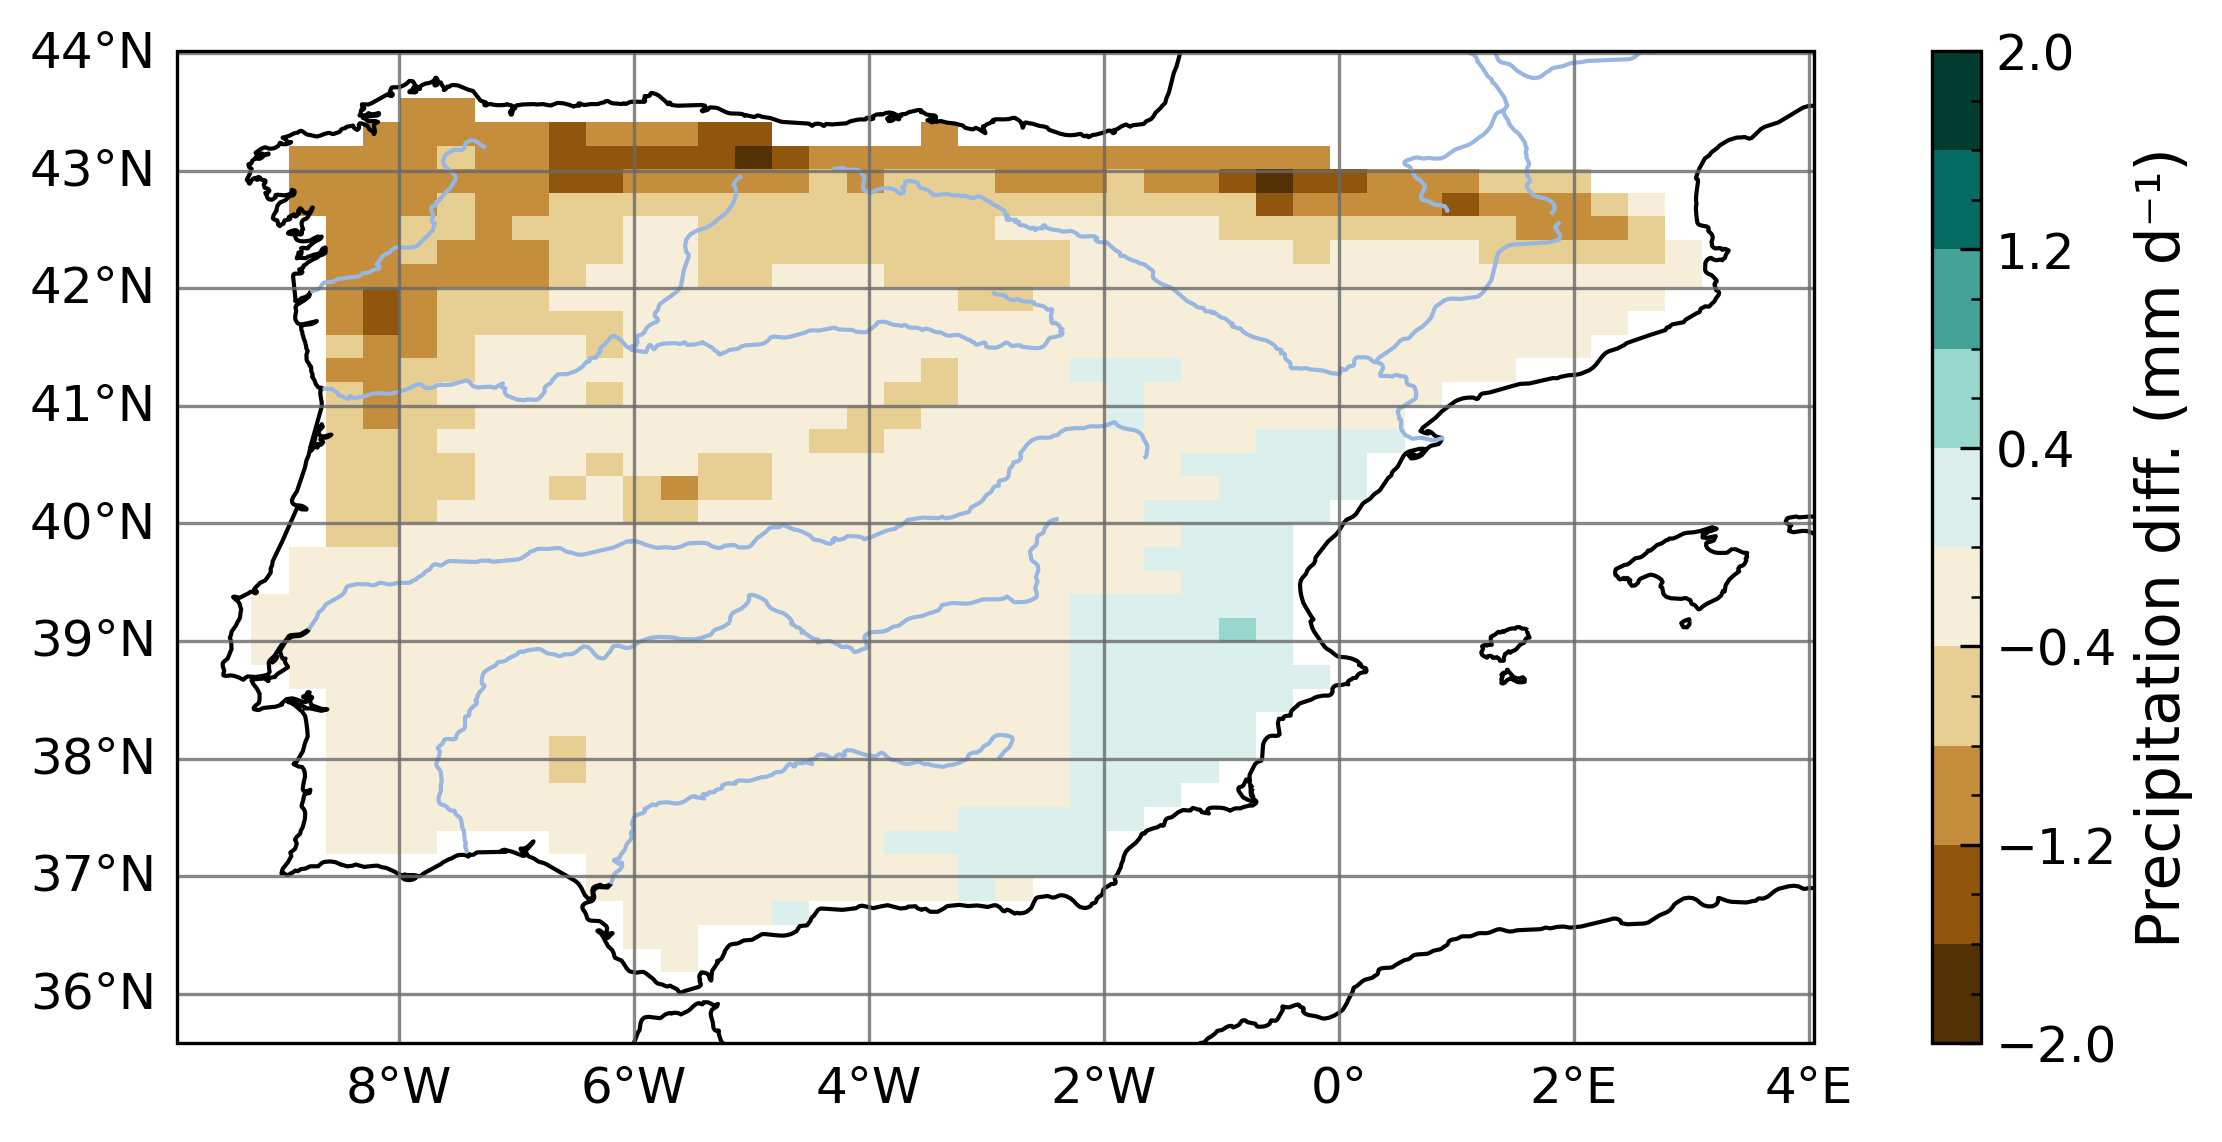
\includegraphics[width=\textwidth]{images/chap4/future/diffmap_precip_presfut.png}
        \end{subfigure} &
        %evap
        \begin{subfigure}[b]{0.5\textwidth}
            \caption{}
            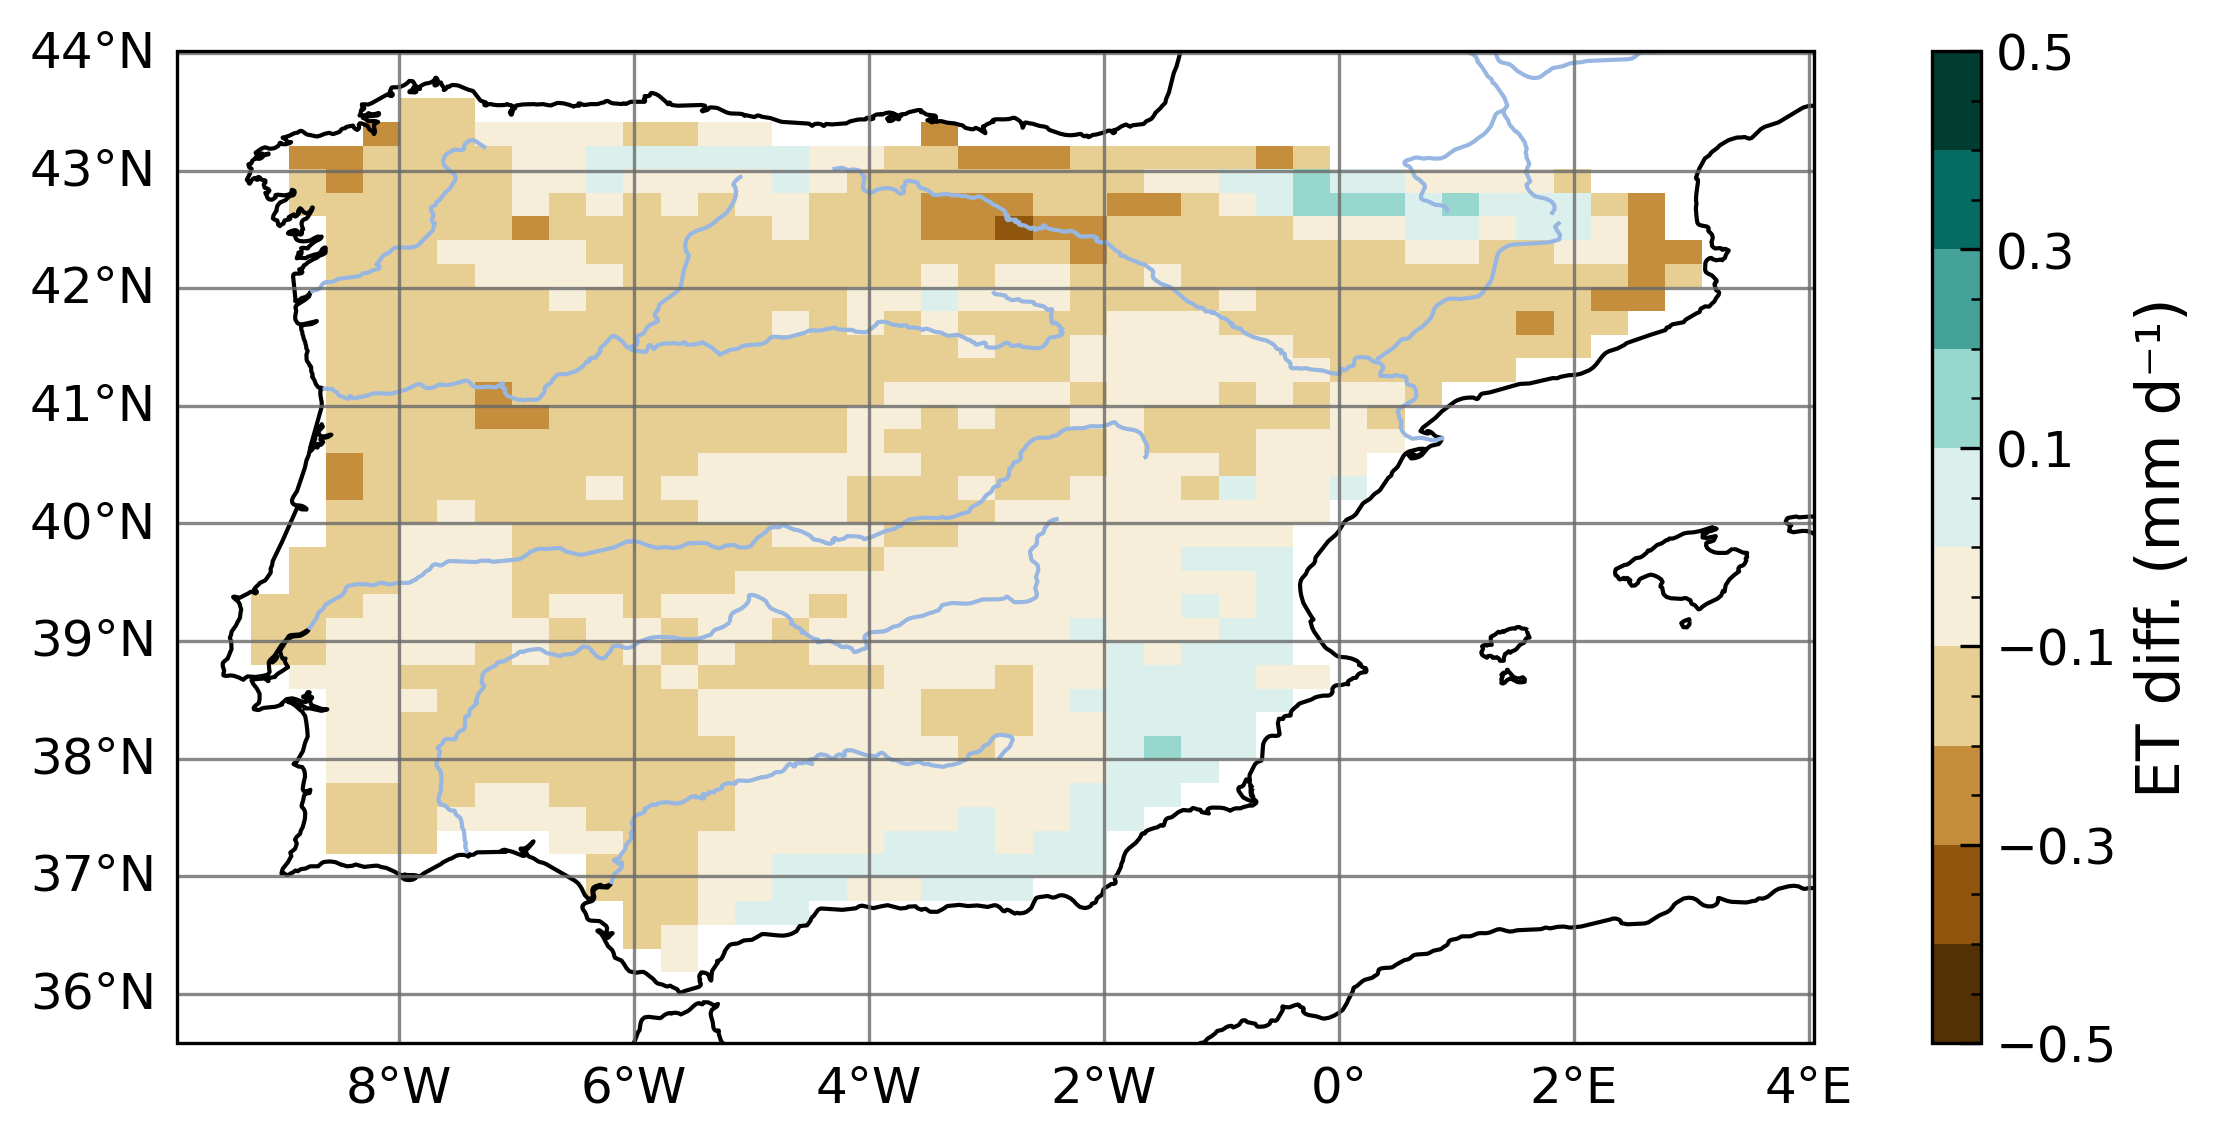
\includegraphics[width=\textwidth]{images/chap4/future/diffmap_evap_presfut.png}
        \end{subfigure} \\

        %t2m
        \begin{subfigure}[b]{0.5\textwidth}
            \caption{}
            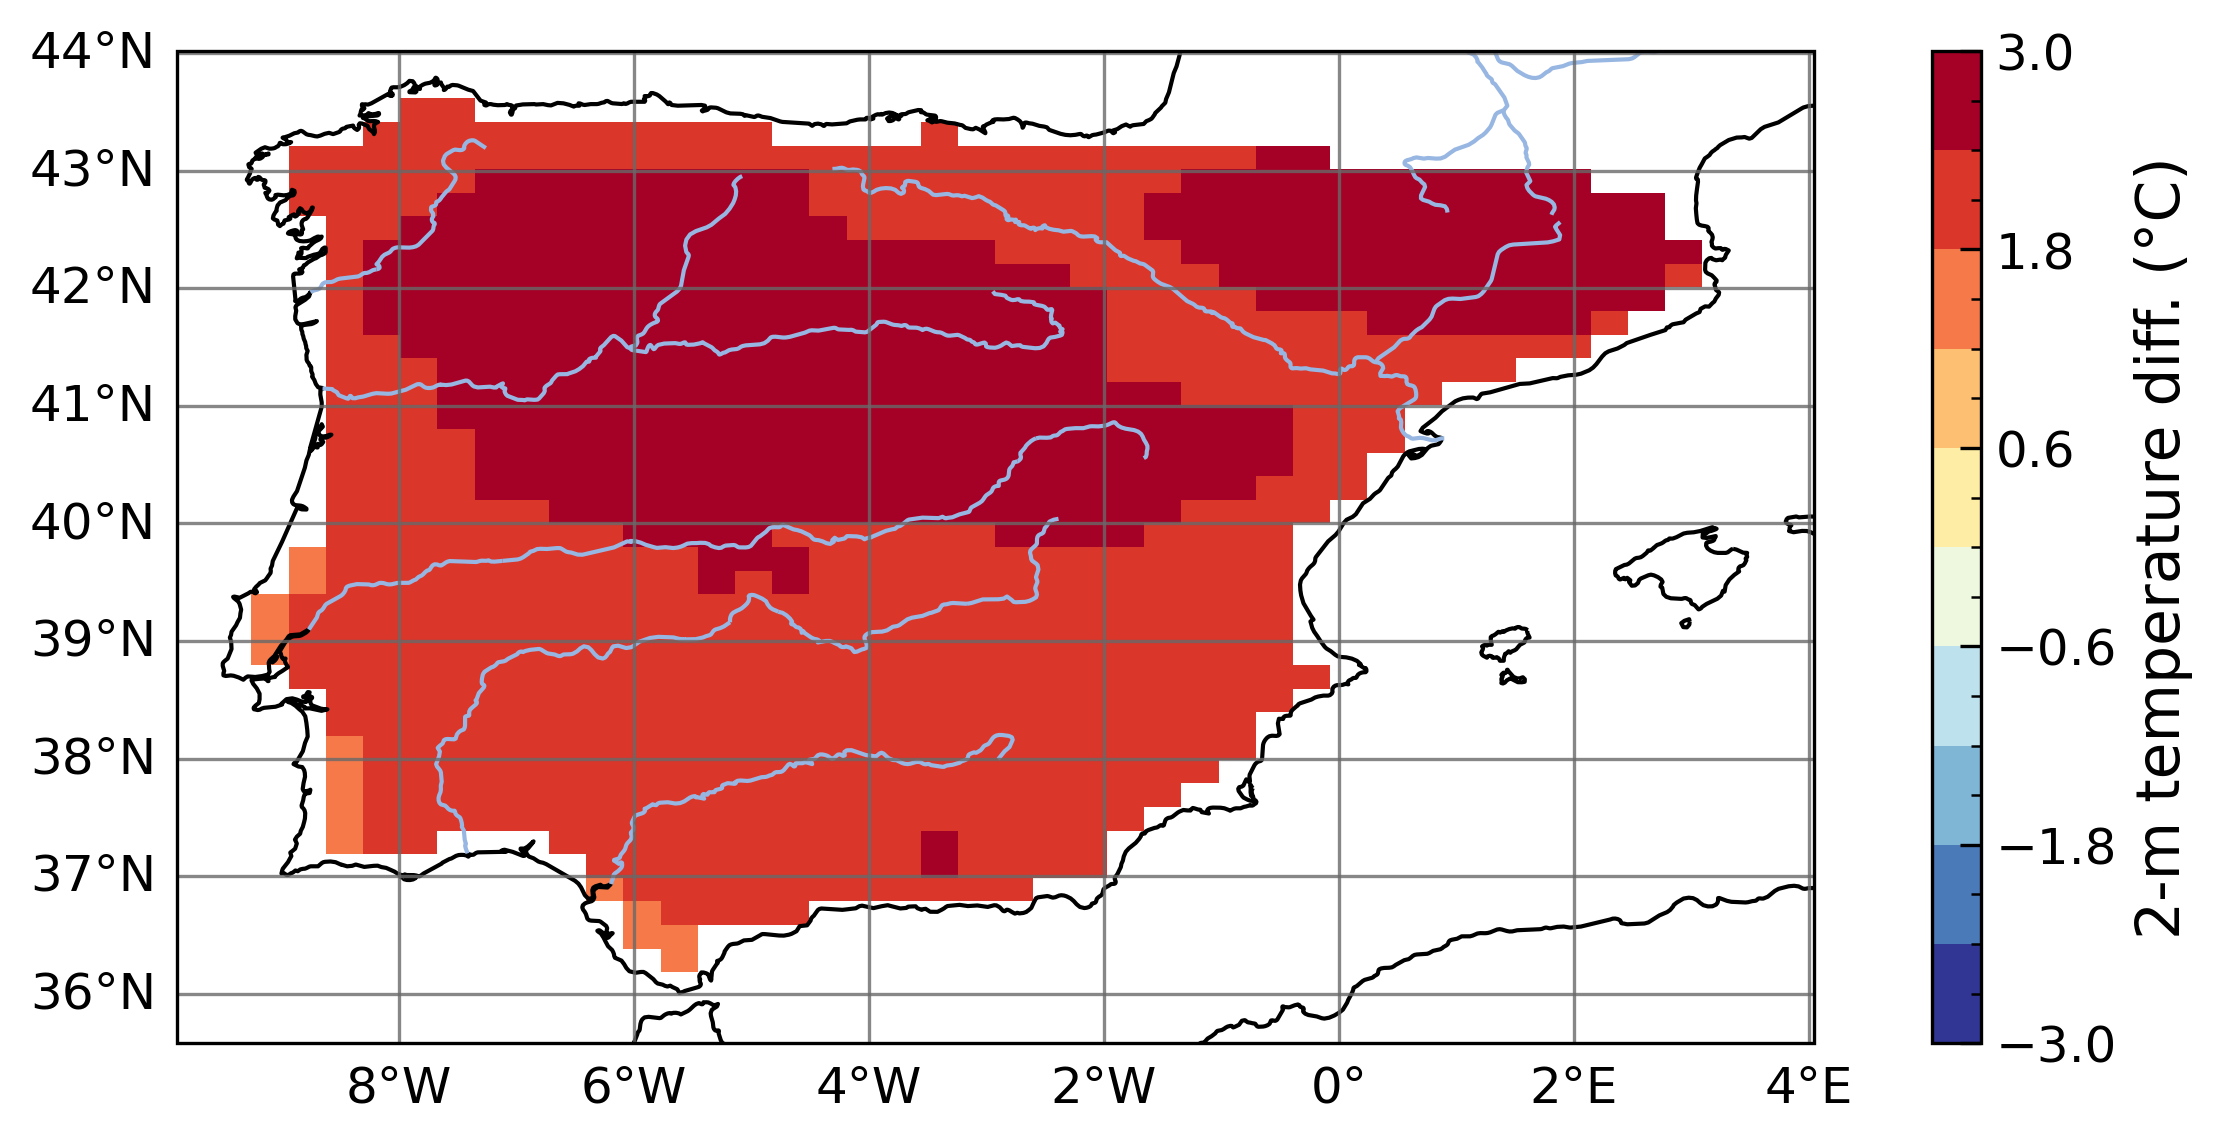
\includegraphics[width=\textwidth]{images/chap4/future/diffmap_t2m_presfut.png}
        \end{subfigure} &
        %fluxsens
        \begin{subfigure}[b]{0.5\textwidth}
            \caption{}
            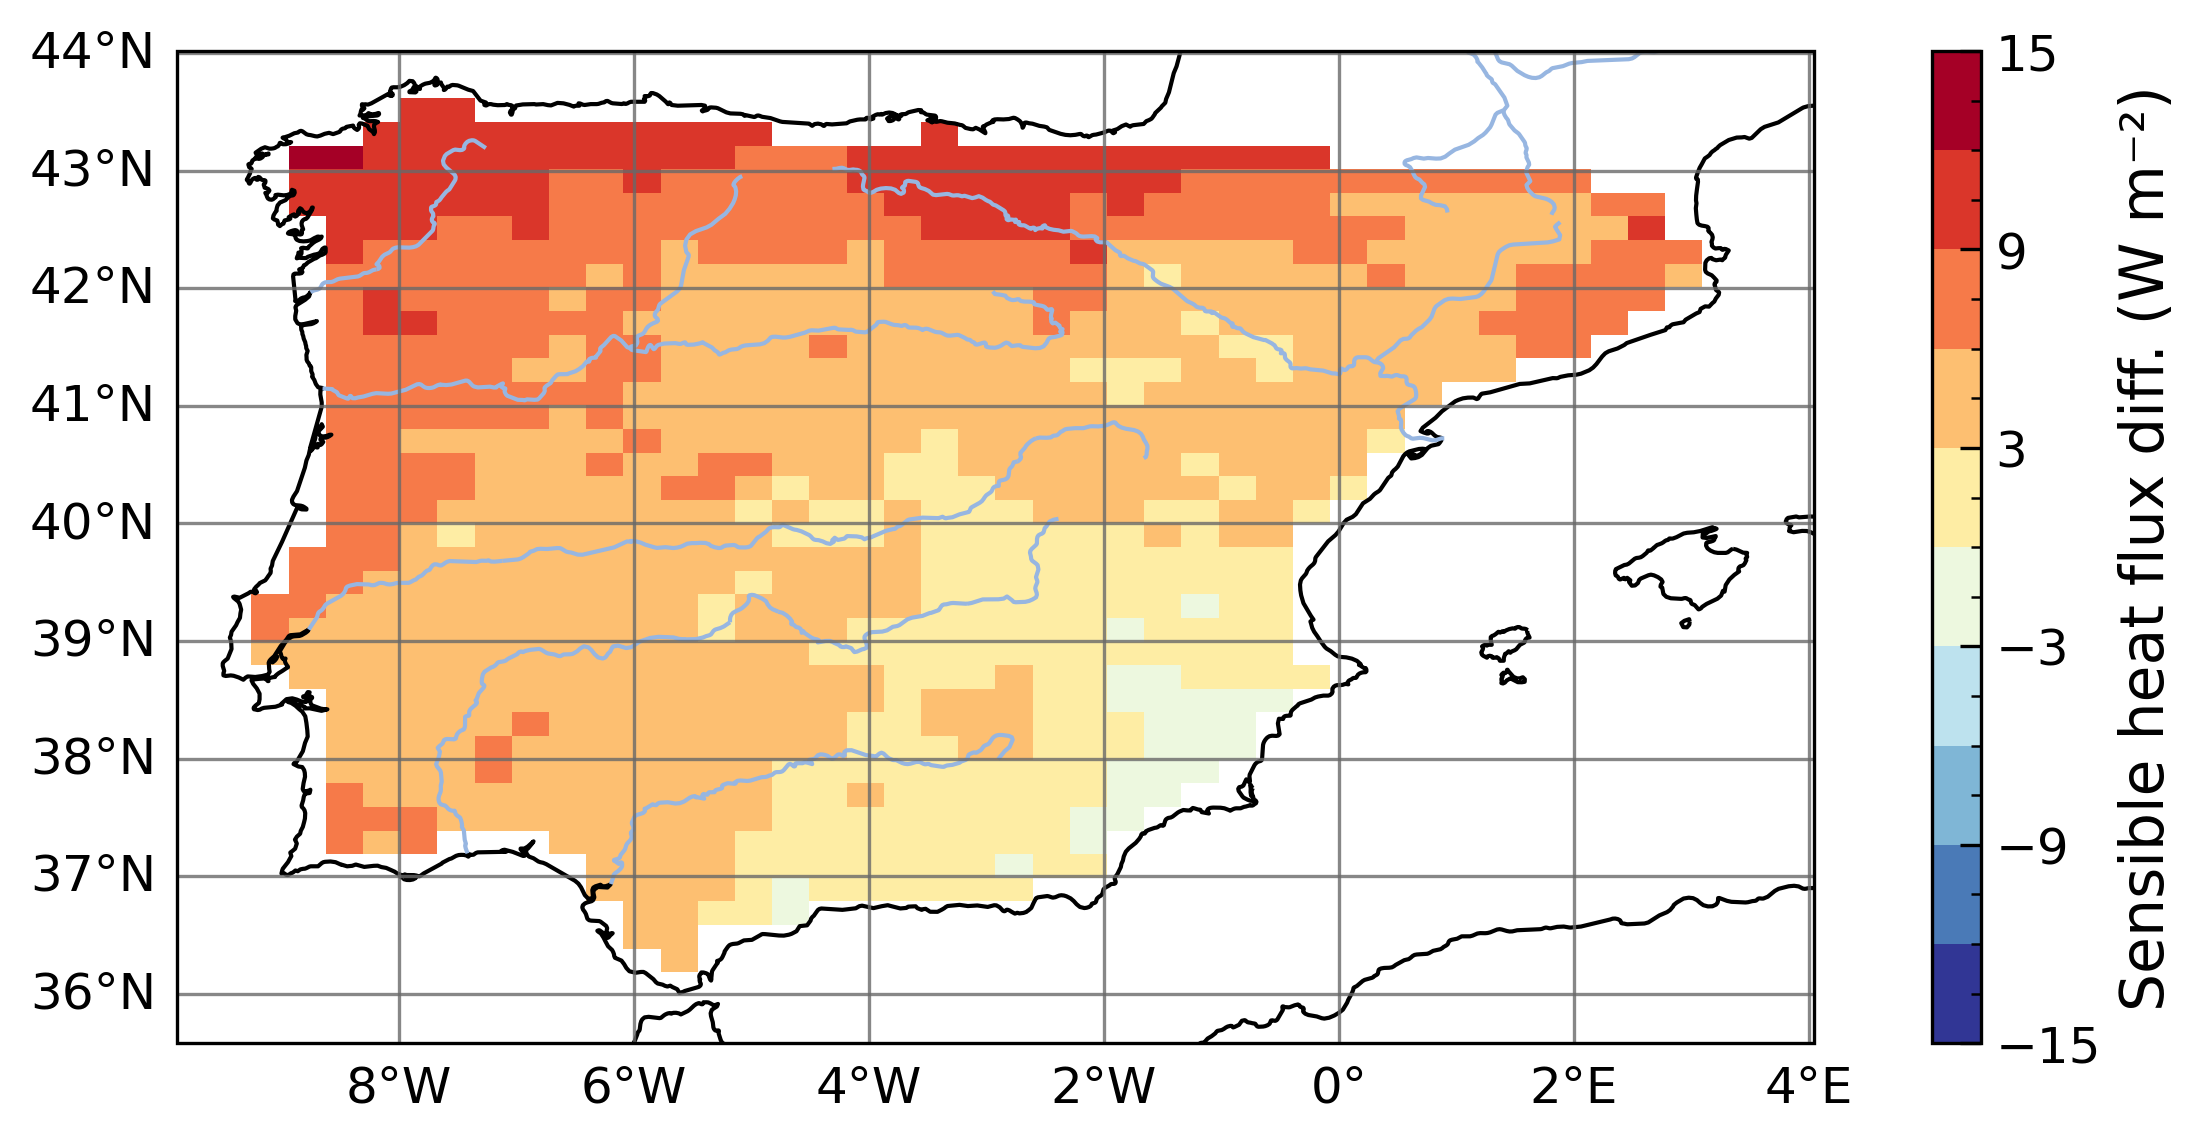
\includegraphics[width=\textwidth]{images/chap4/future/diffmap_fluxsens_presfut.png}
        \end{subfigure} \\

        %q2m
        \begin{subfigure}[b]{0.5\textwidth}
            \caption{}
            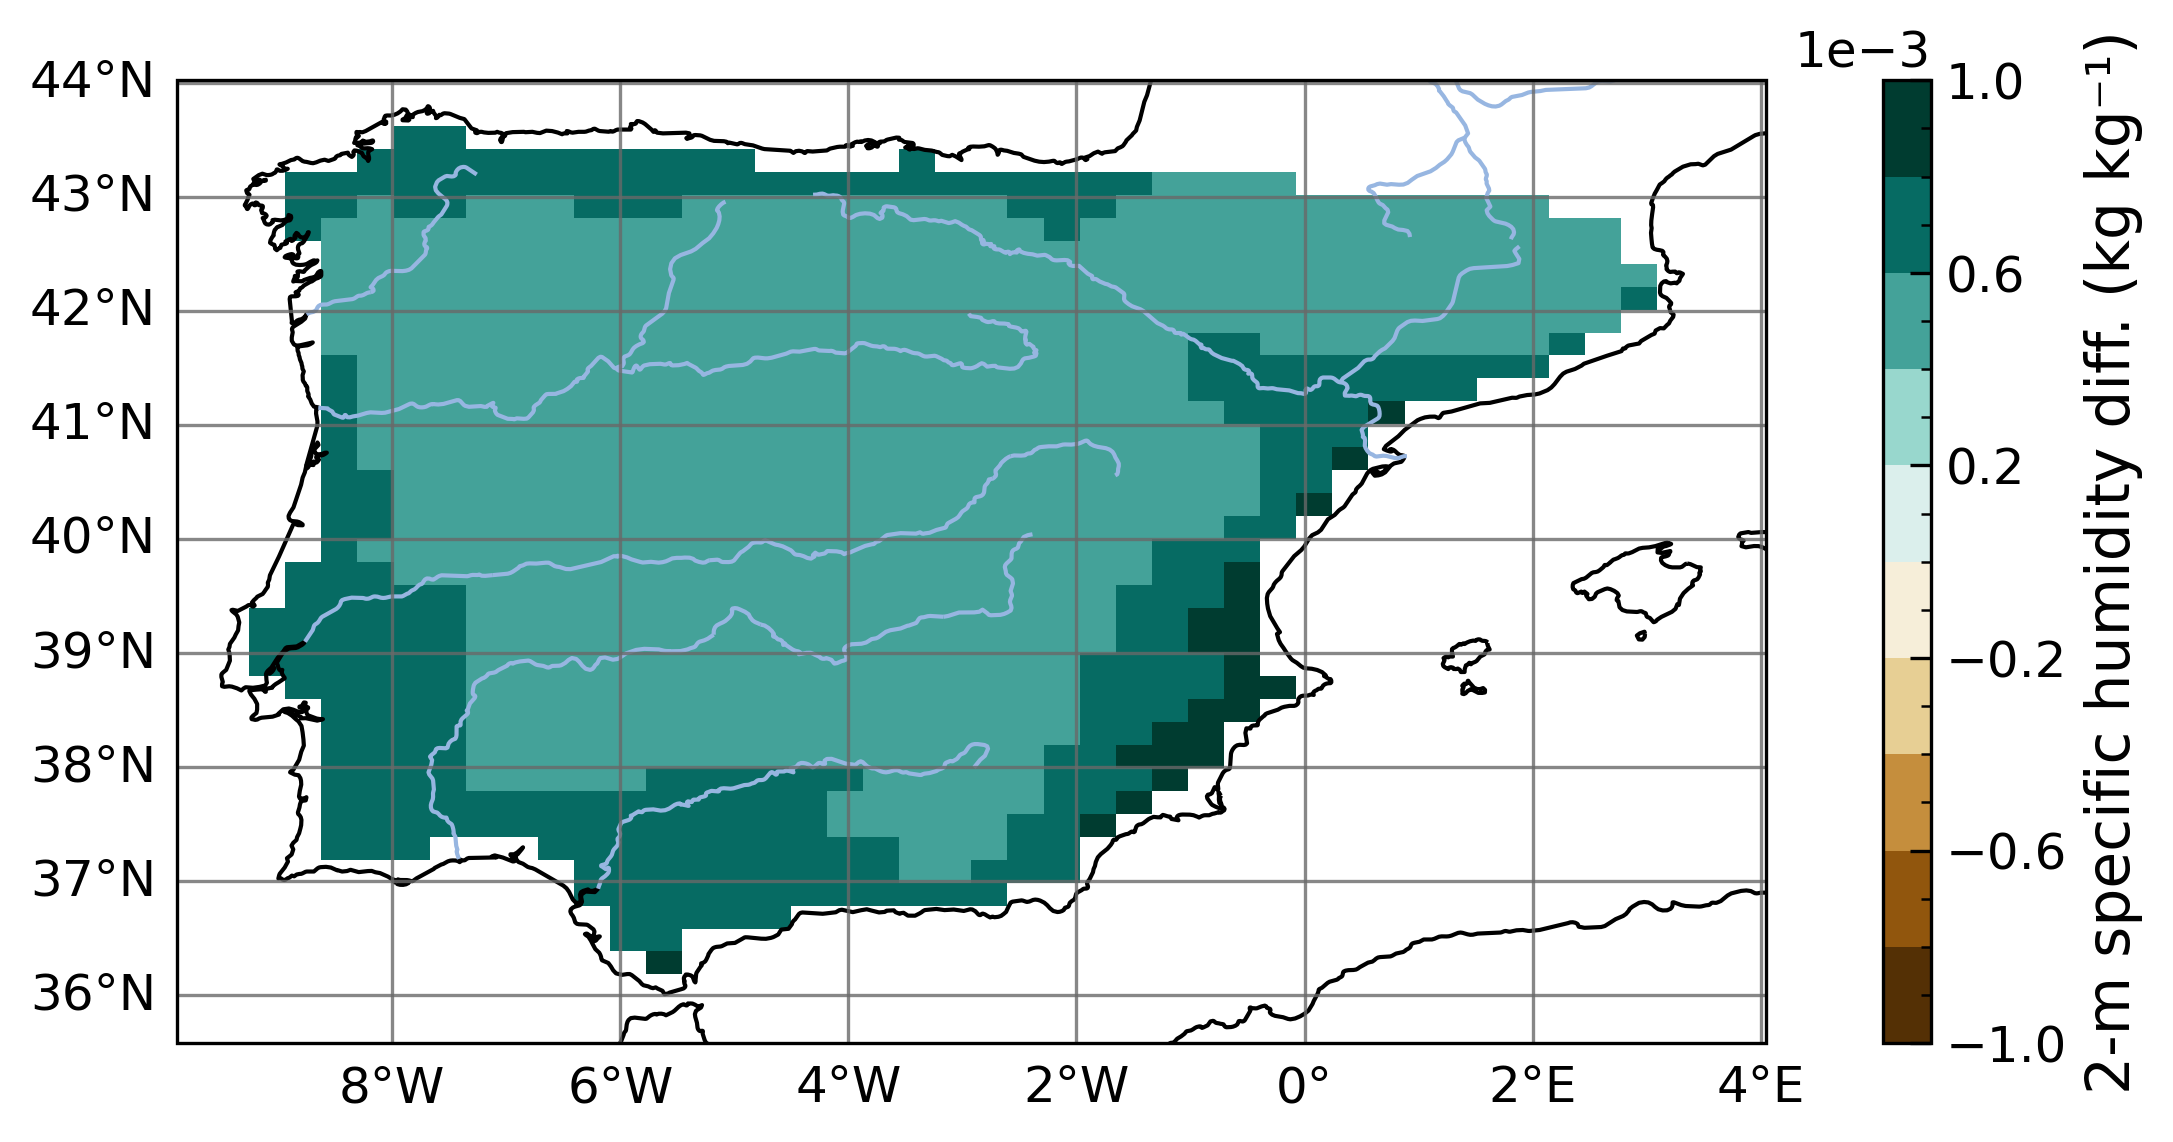
\includegraphics[width=\textwidth]{images/chap4/future/diffmap_q2m_presfut.png}
        \end{subfigure} &
        %rh2m
        \begin{subfigure}[b]{0.5\textwidth}
            \caption{}
            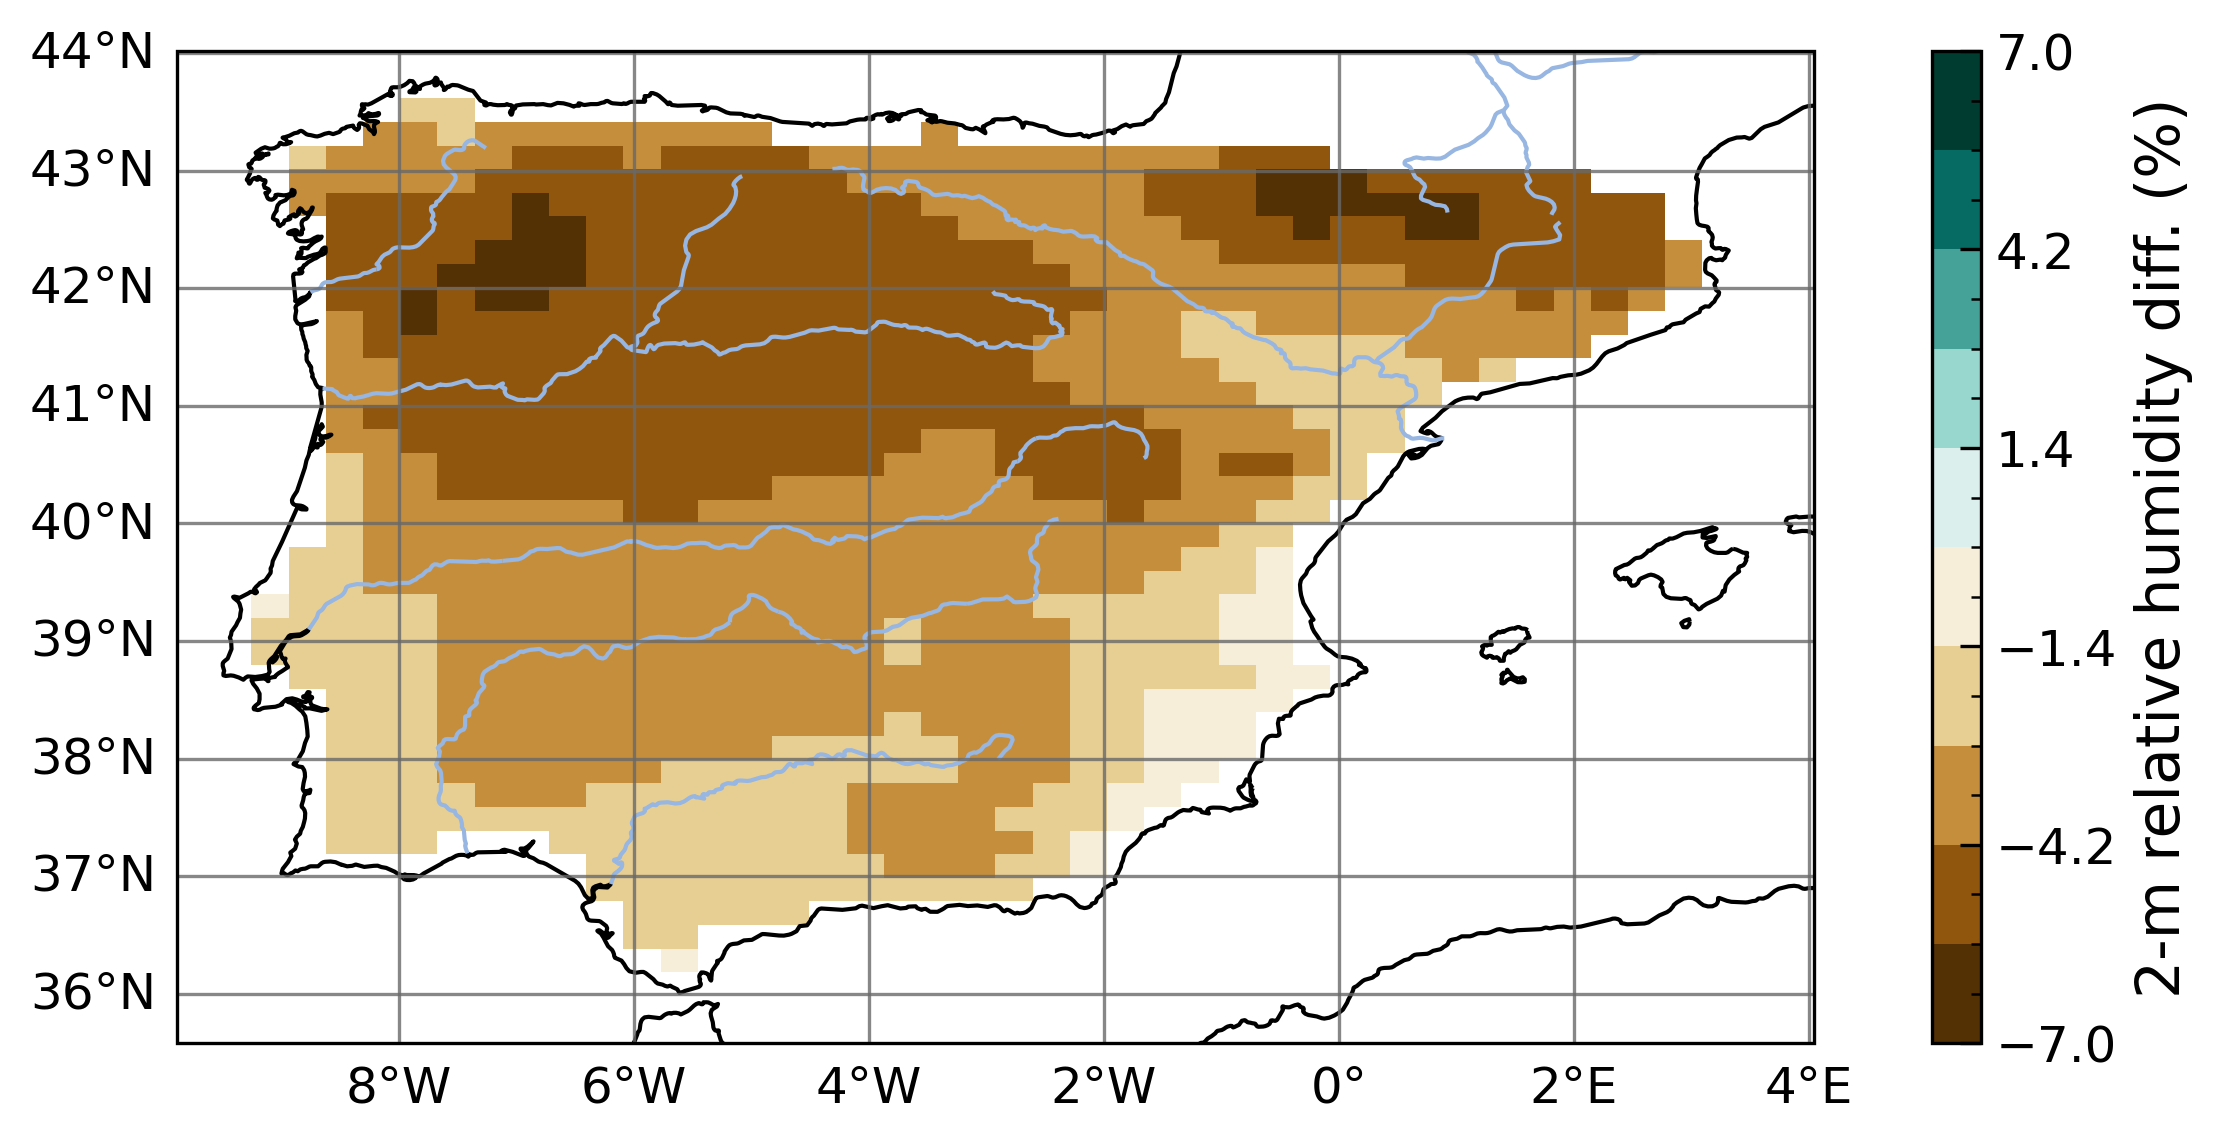
\includegraphics[width=\textwidth]{images/chap4/future/diffmap_rh2m_presfut.png}
        \end{subfigure} \\

        %pblh
        \begin{subfigure}[b]{0.5\textwidth}
            \caption{}
            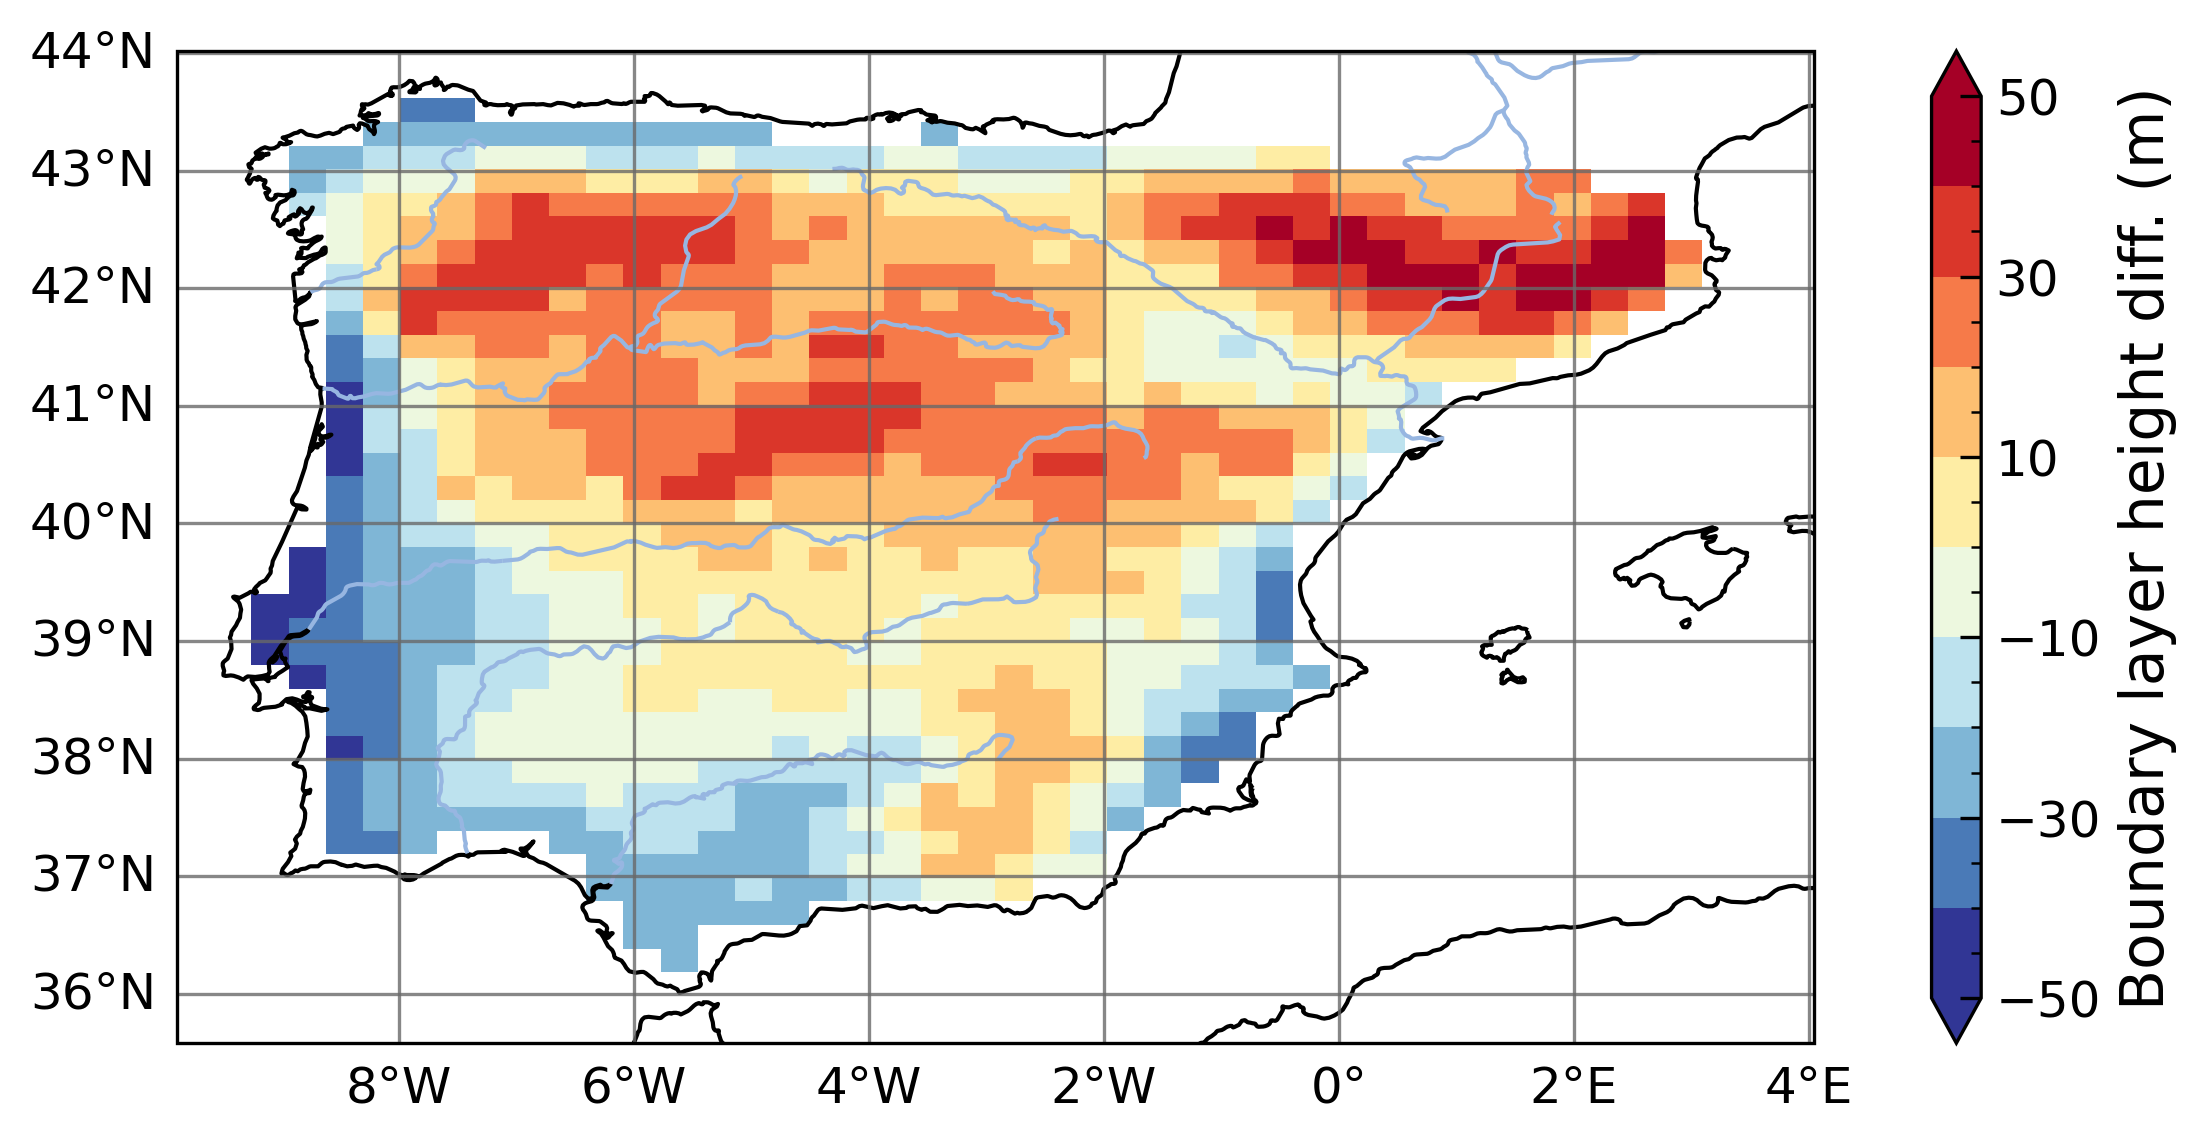
\includegraphics[width=\textwidth]{images/chap4/future/diffmap_s_pblh_presfut.png}
        \end{subfigure} &
        %lcl
        \begin{subfigure}[b]{0.5\textwidth}
            \caption{}
            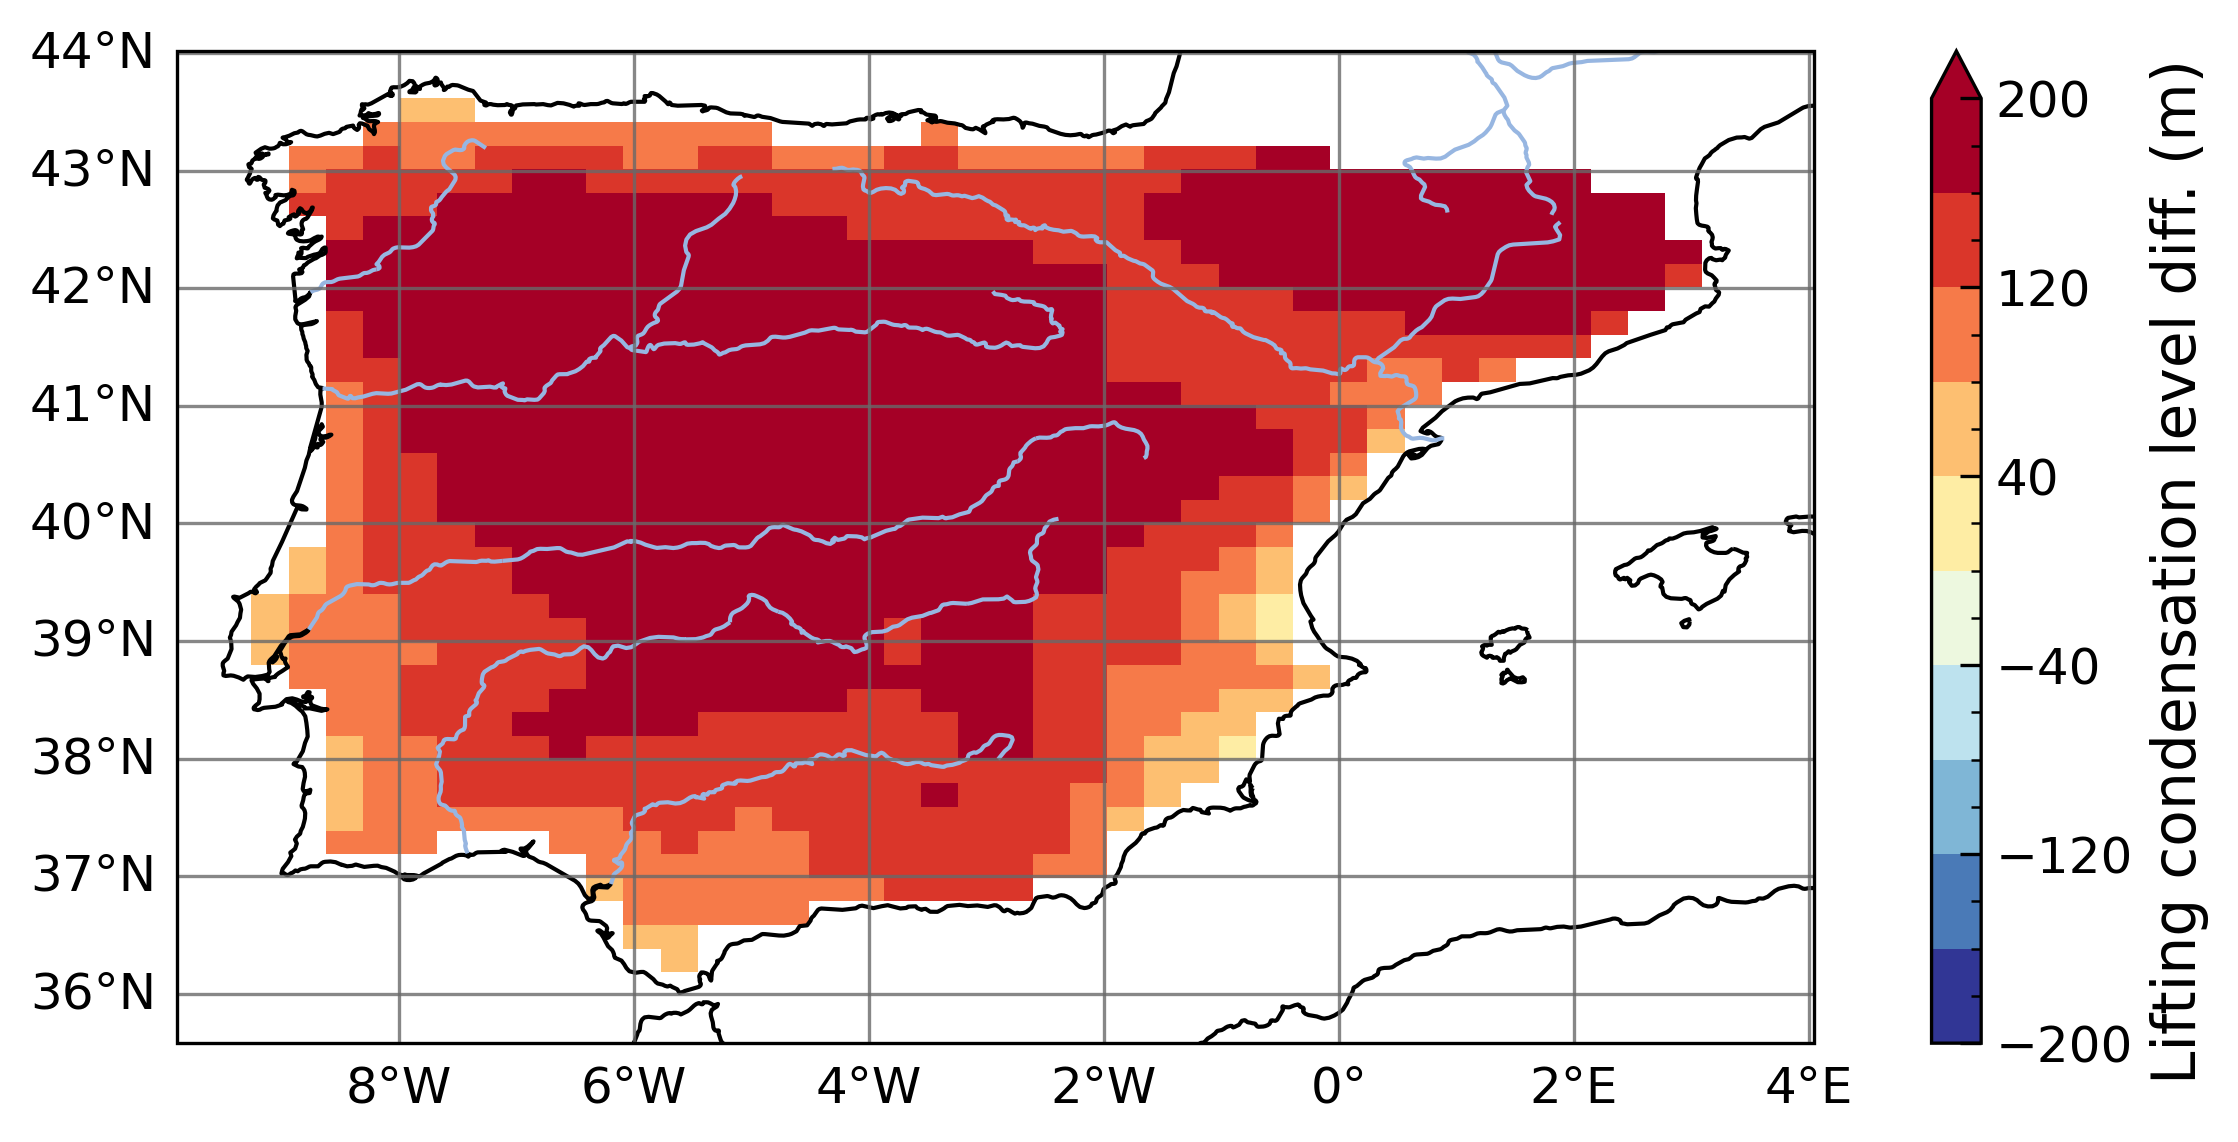
\includegraphics[width=\textwidth]{images/chap4/future/diffmap_s_lcl_presfut.png}
        \end{subfigure} \\
    \end{tabular}
    \caption{}
    \label{fig:diffmaps_present_future}
\end{figure}

\clearpage

\subsection{Modulation of climate change by irrigation}

%figure : map as SC of irrigation in the future
\begin{figure}[htbp]
    \centering
    \begin{tabular}{cc}
        %precip
        \begin{subfigure}[b]{0.48\textwidth}
            \caption{}
            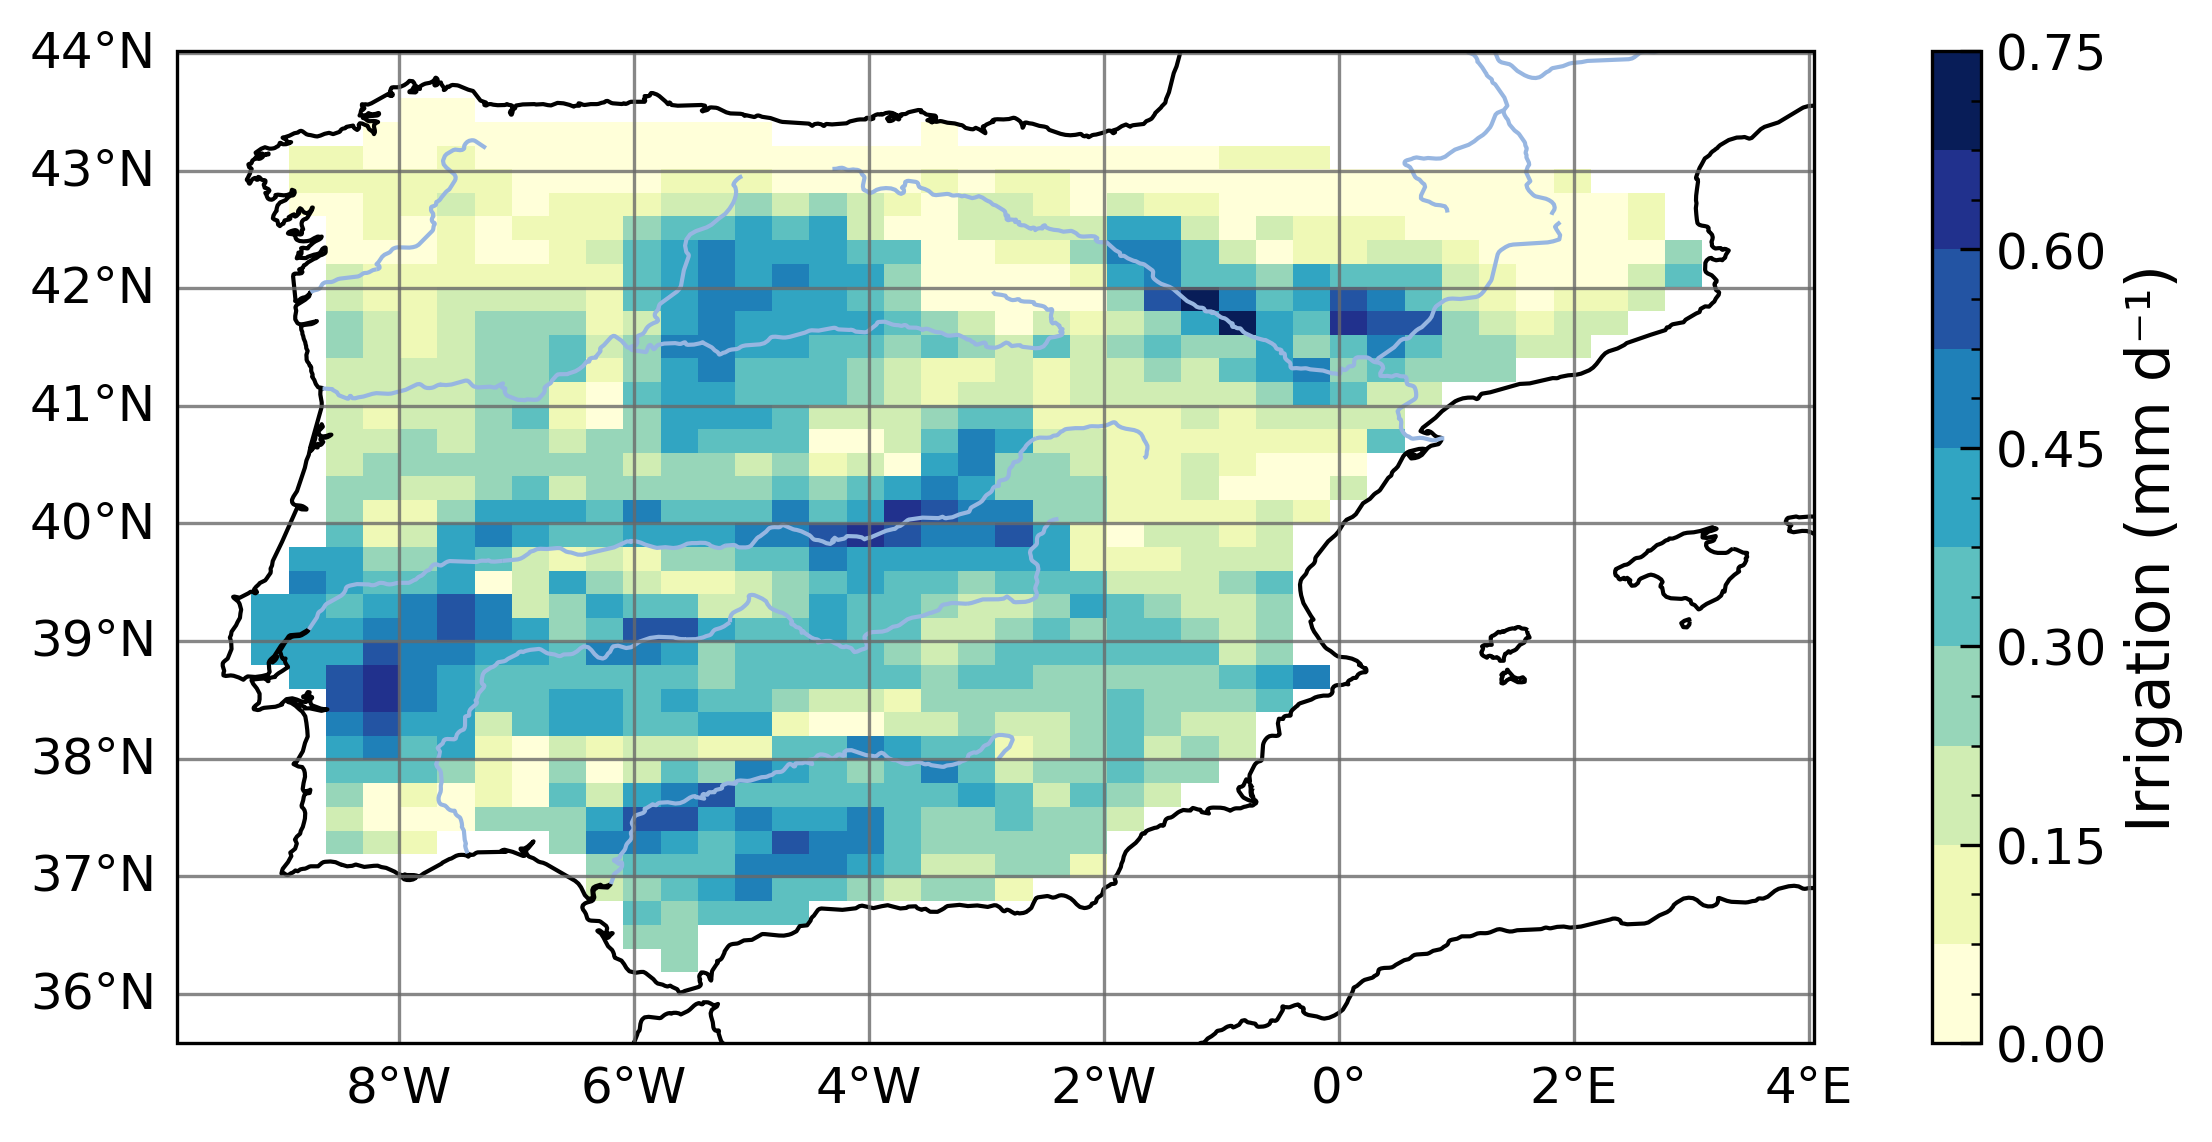
\includegraphics[width=\textwidth]{images/chap4/future/map_irrigation_fut.png}
        \end{subfigure} &
        \begin{subfigure}[b]{0.46\textwidth}
            \caption{}
            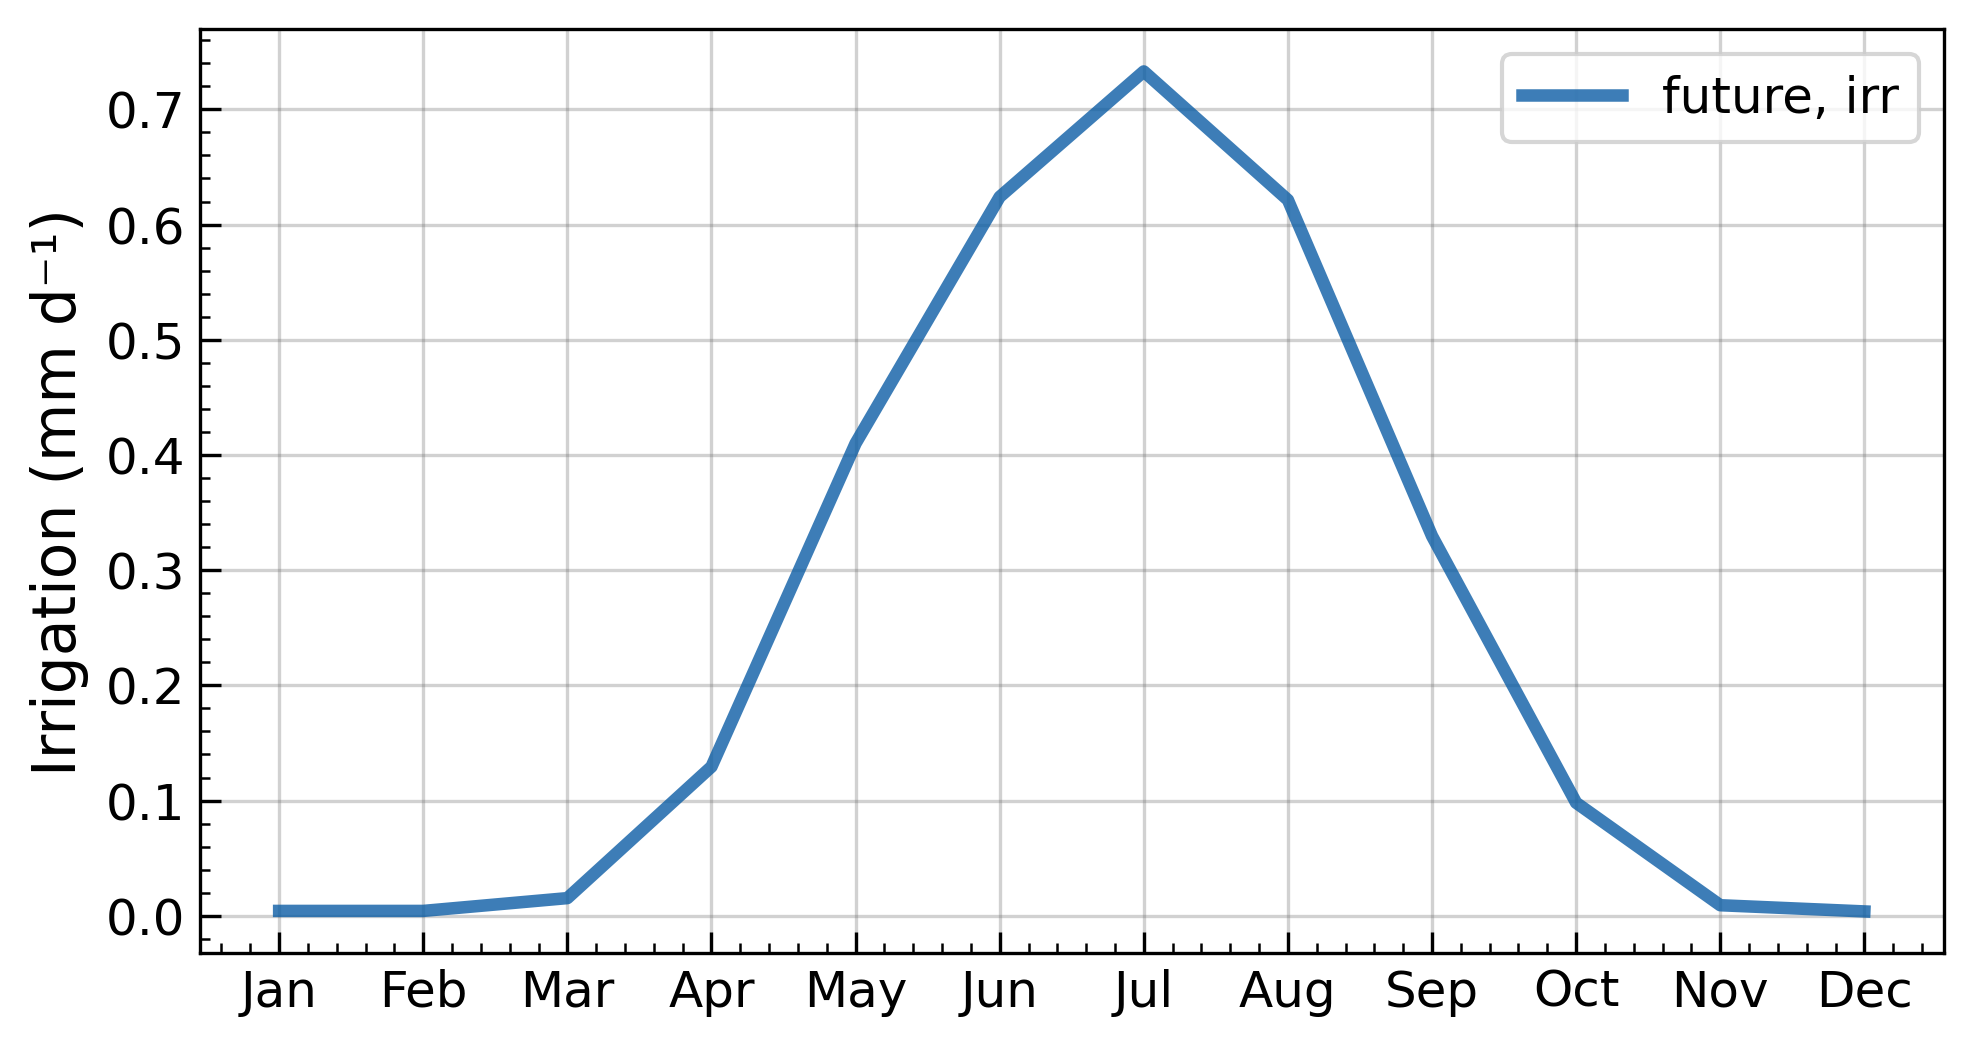
\includegraphics[width=\textwidth]{images/chap4/future/SC_irrigation_fut.png}
        \end{subfigure}
    \end{tabular}
    \caption{}
    \label{fig:future_irrig}
\end{figure}

%figure : diff maps (future, irr - no_irr)
\begin{figure}[htbp]
    \centering
    \begin{tabular}{cc}
        %precip
        \begin{subfigure}[b]{0.5\textwidth}
            \caption{}
            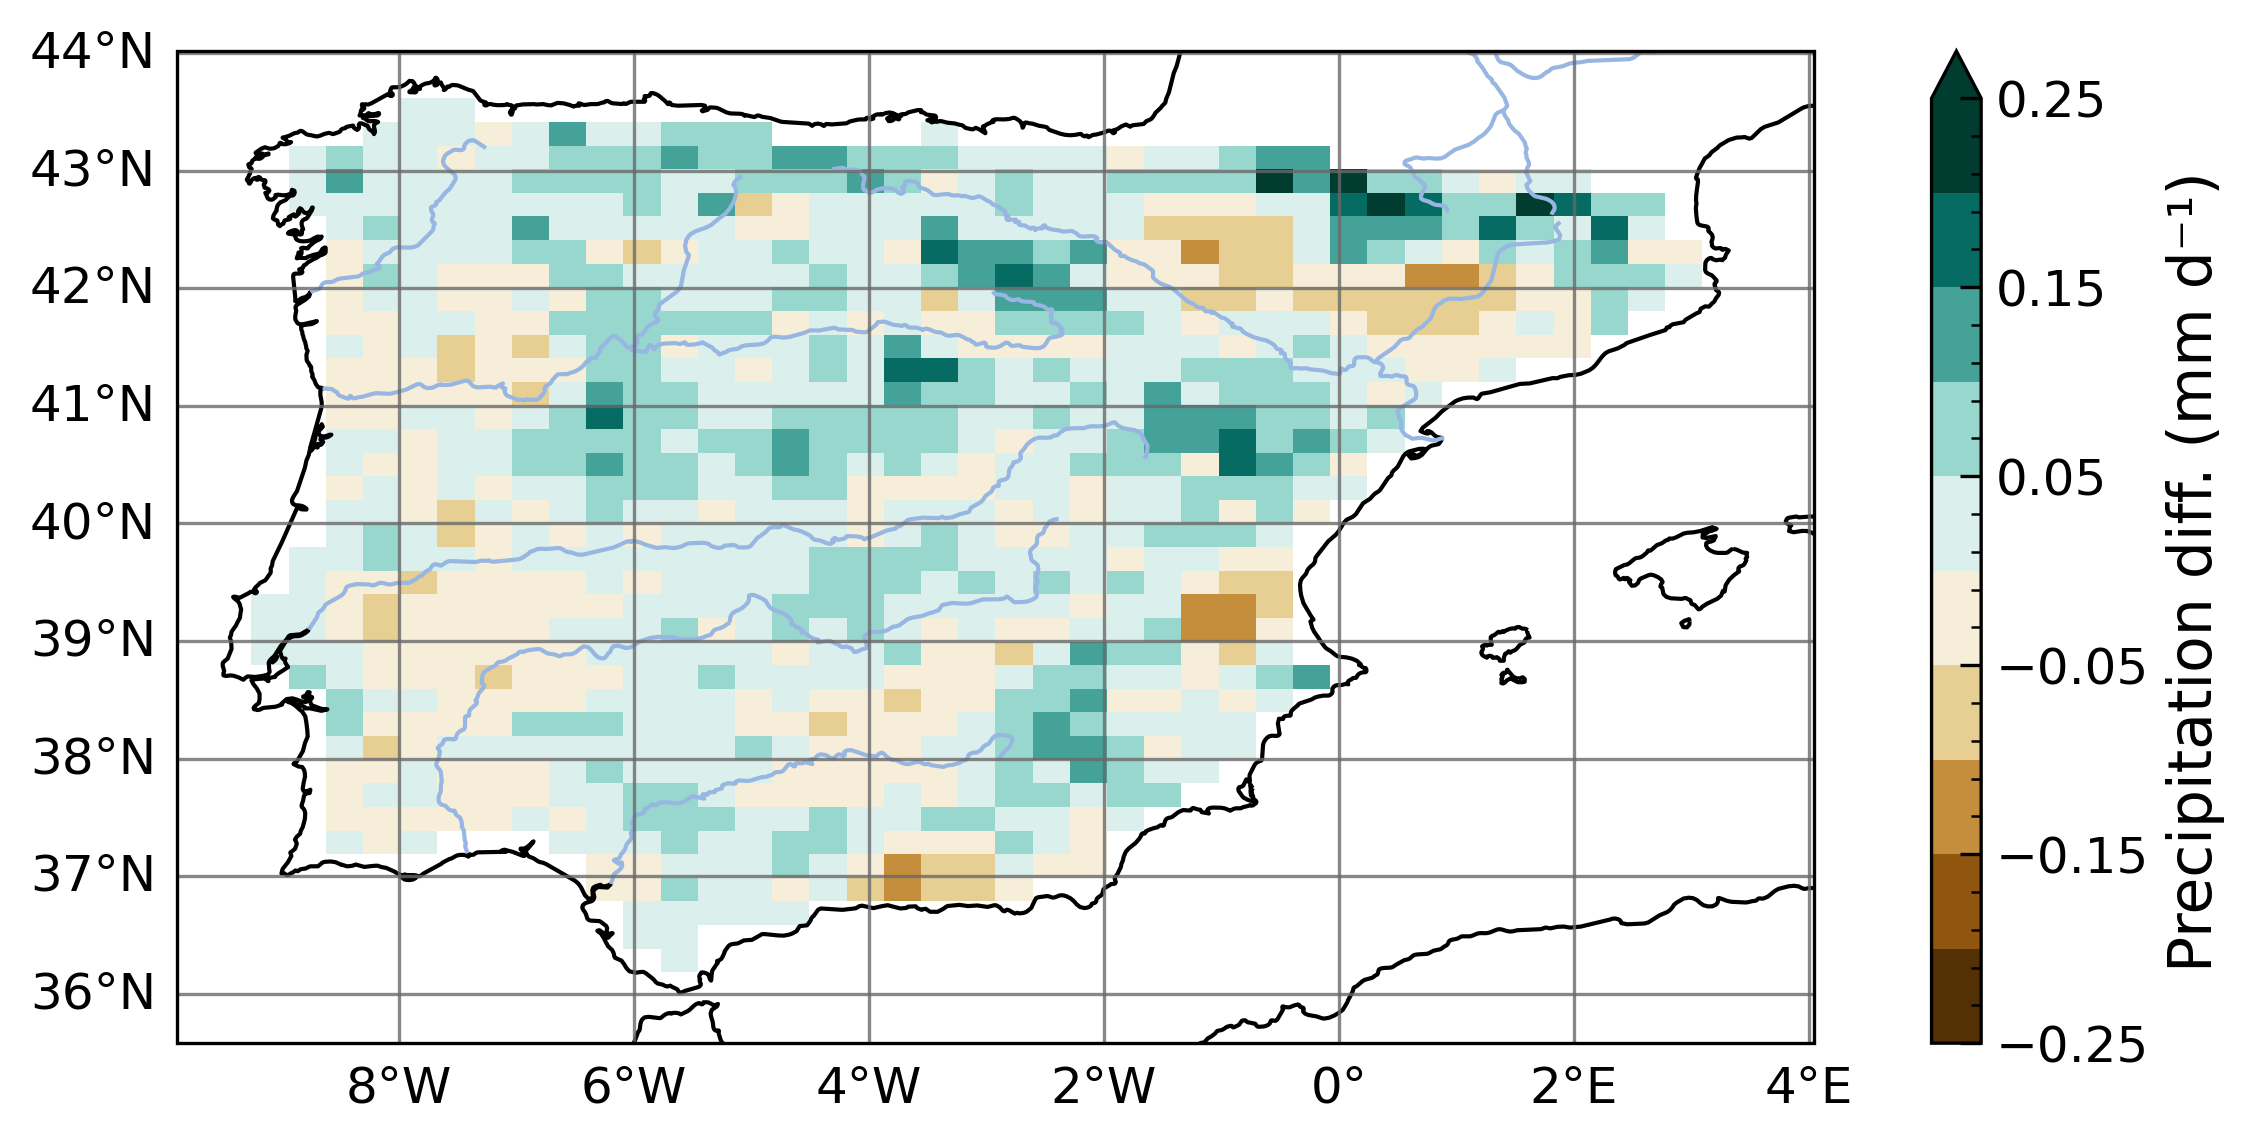
\includegraphics[width=\textwidth]{images/chap4/future/diffmap_precip_futirr.png}
        \end{subfigure} &
        %evap
        \begin{subfigure}[b]{0.5\textwidth}
            \caption{}
            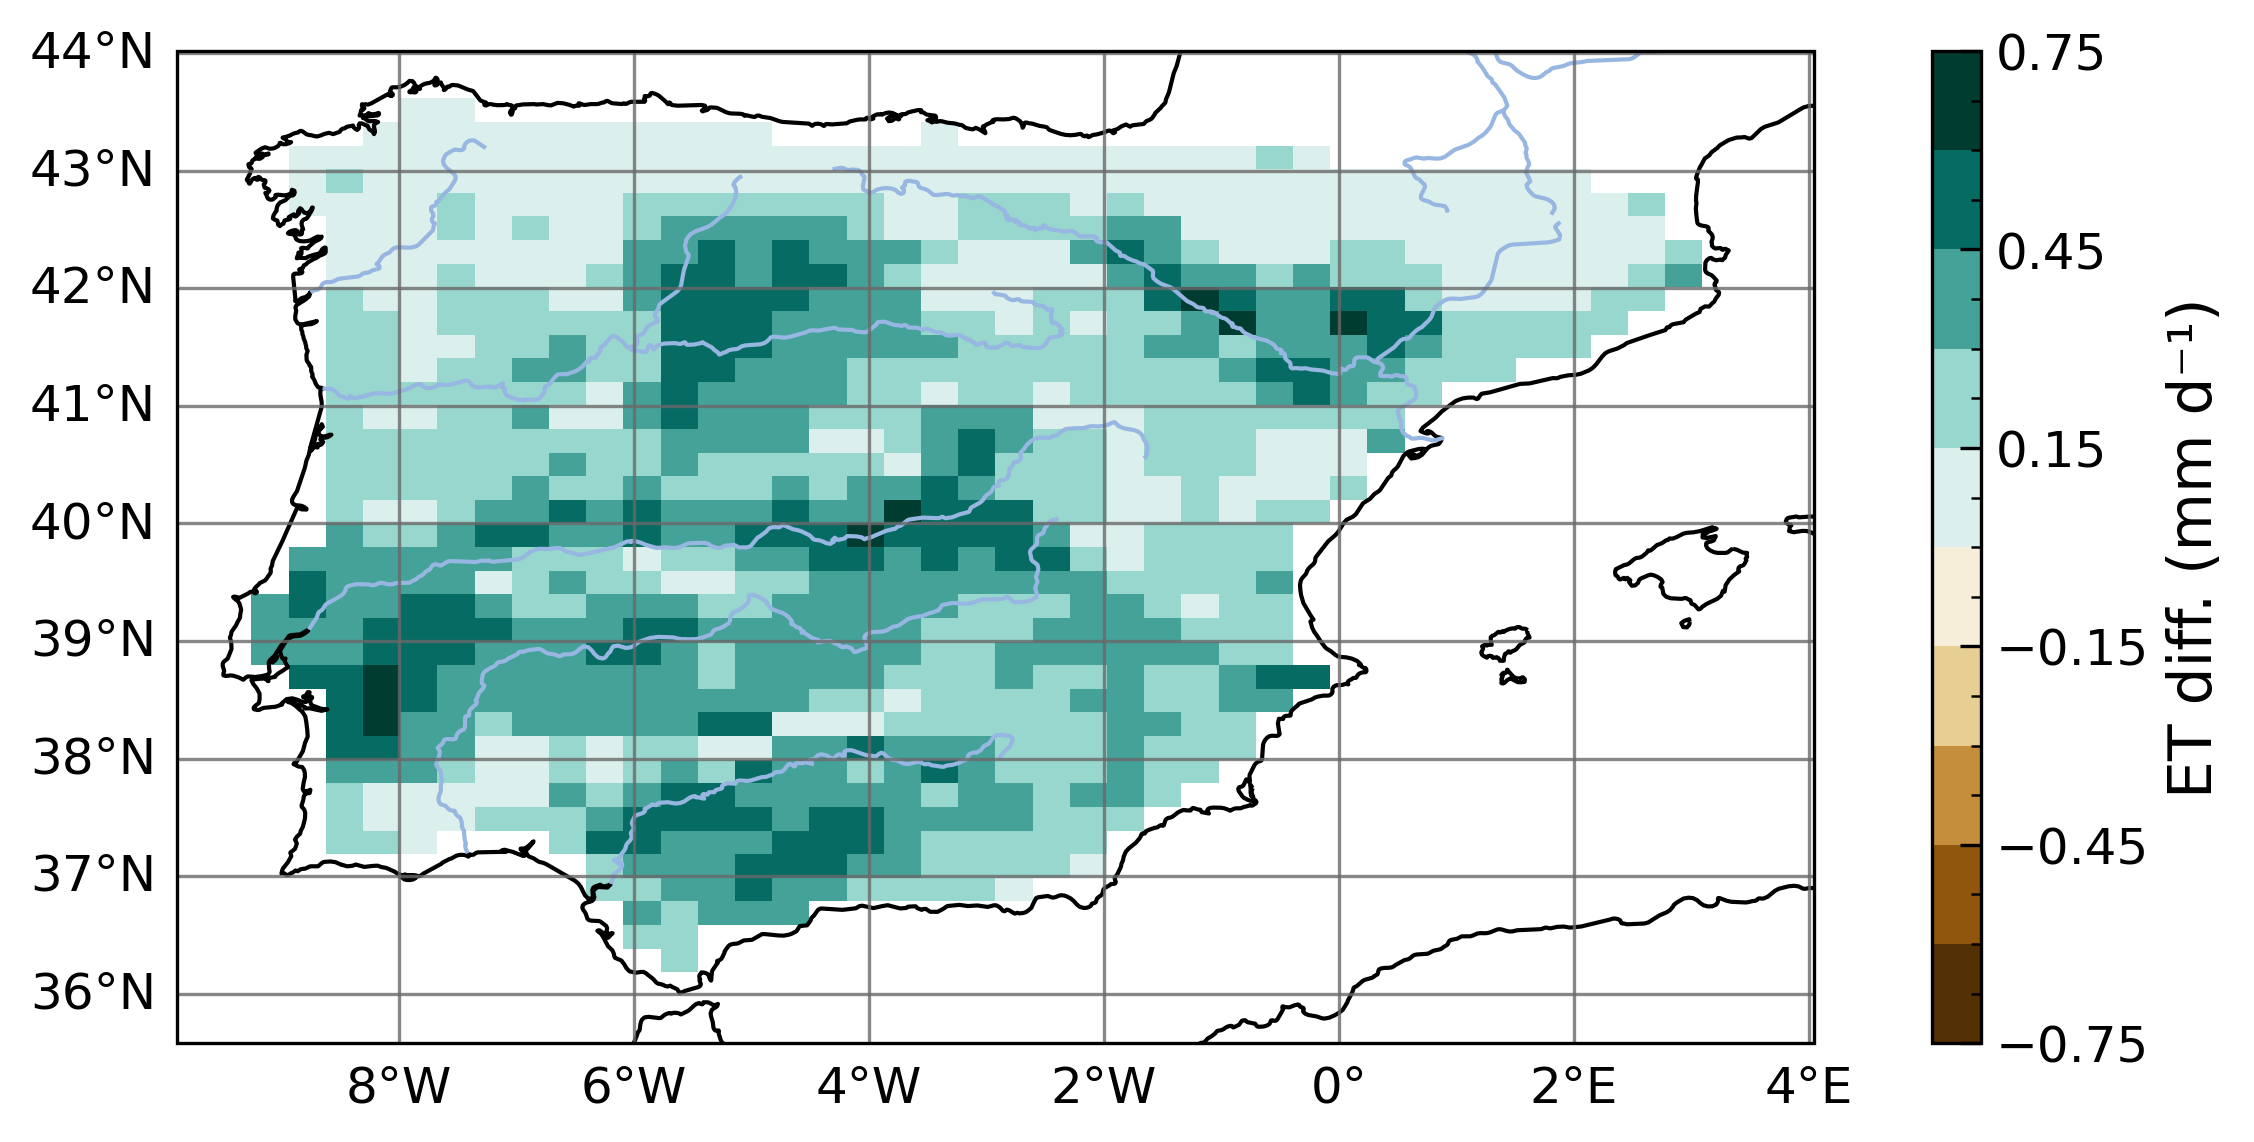
\includegraphics[width=\textwidth]{images/chap4/future/diffmap_evap_futirr.png}
        \end{subfigure} \\

        %t2m
        \begin{subfigure}[b]{0.5\textwidth}
            \caption{}
            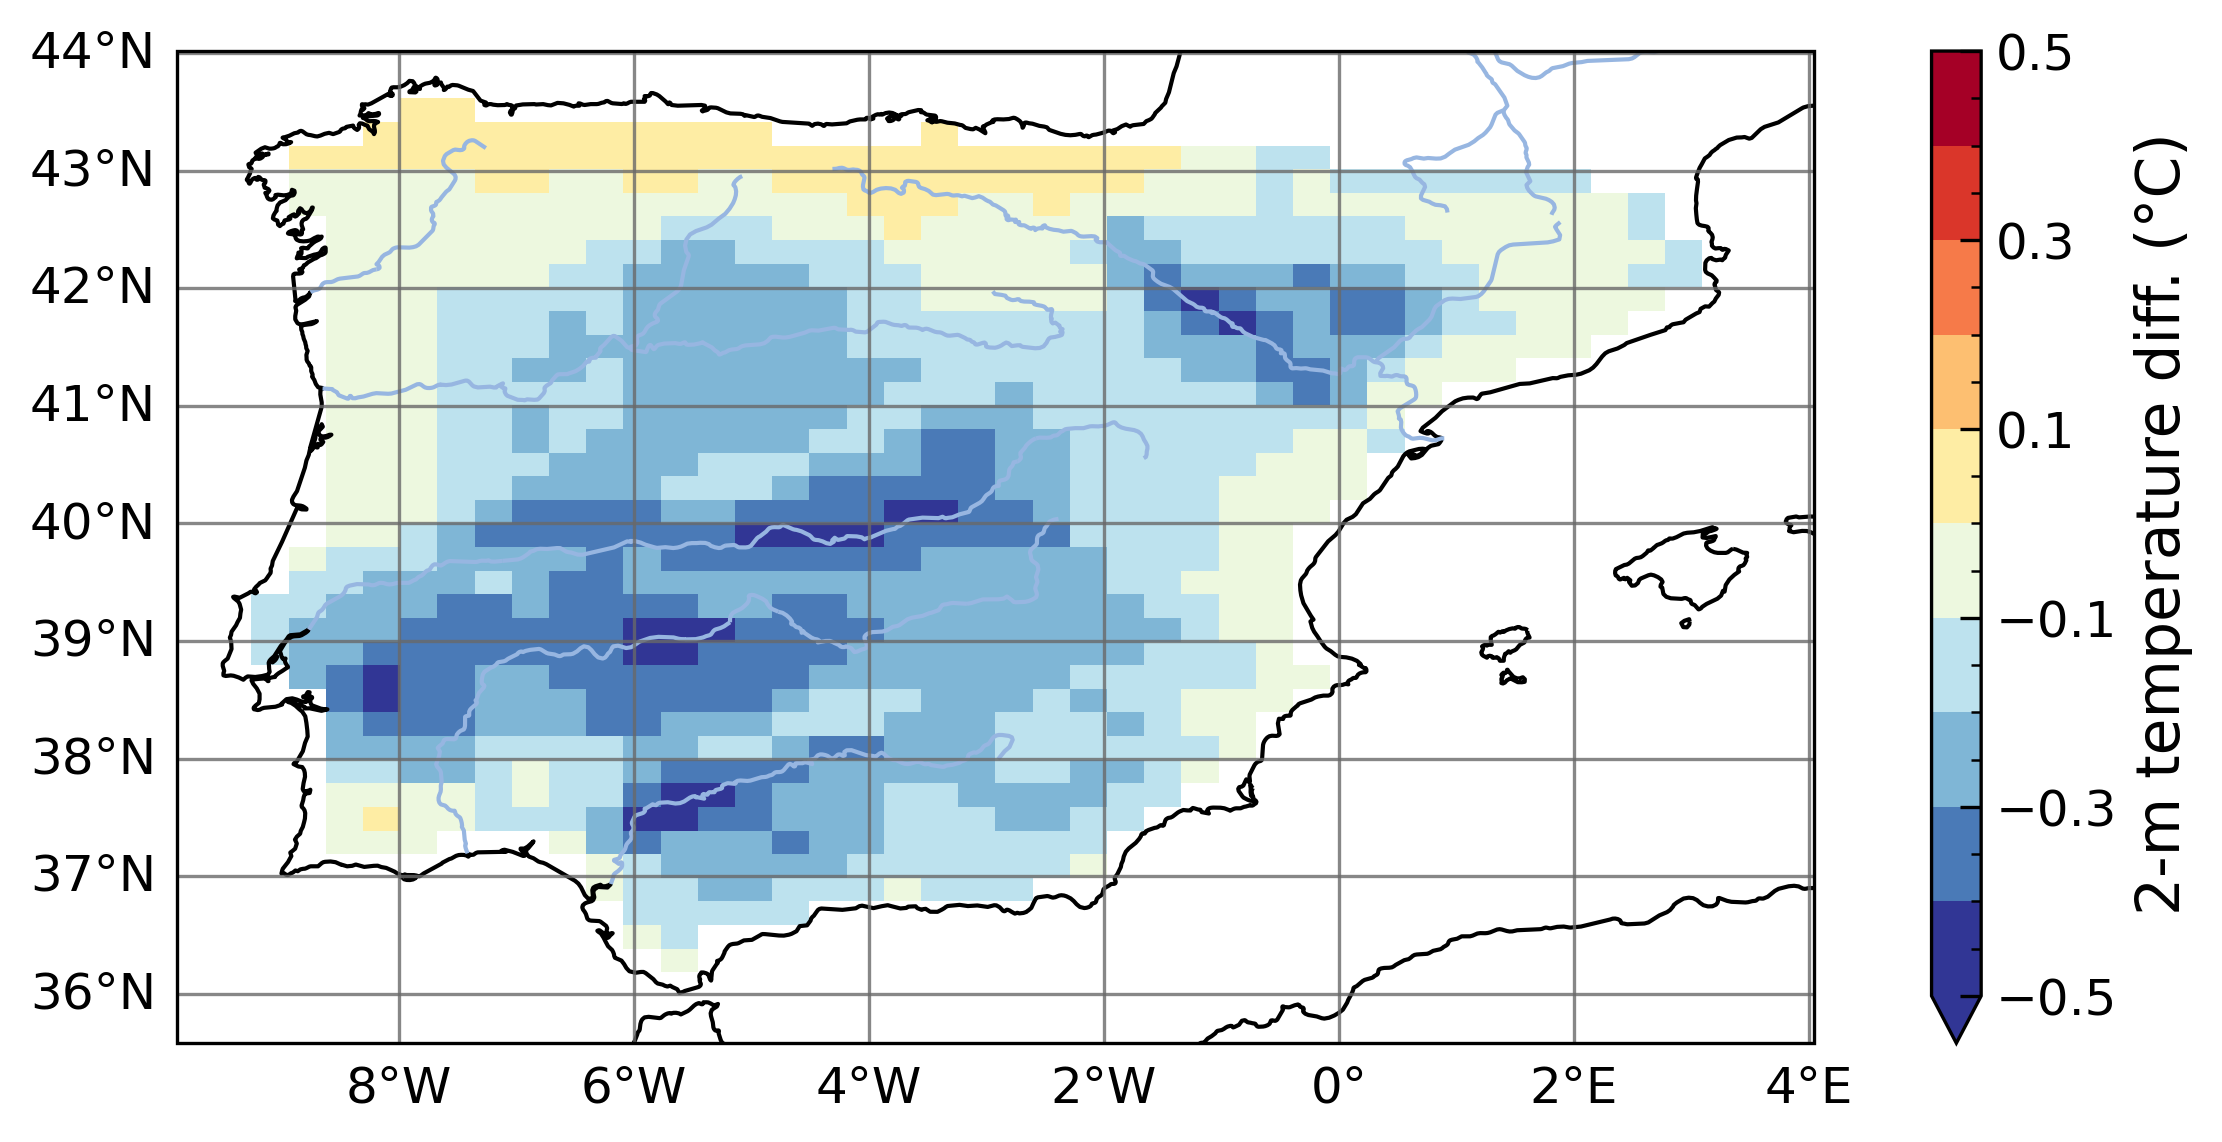
\includegraphics[width=\textwidth]{images/chap4/future/diffmap_t2m_futirr.png}
        \end{subfigure} &
        %fluxsens
        \begin{subfigure}[b]{0.5\textwidth}
            \caption{}
            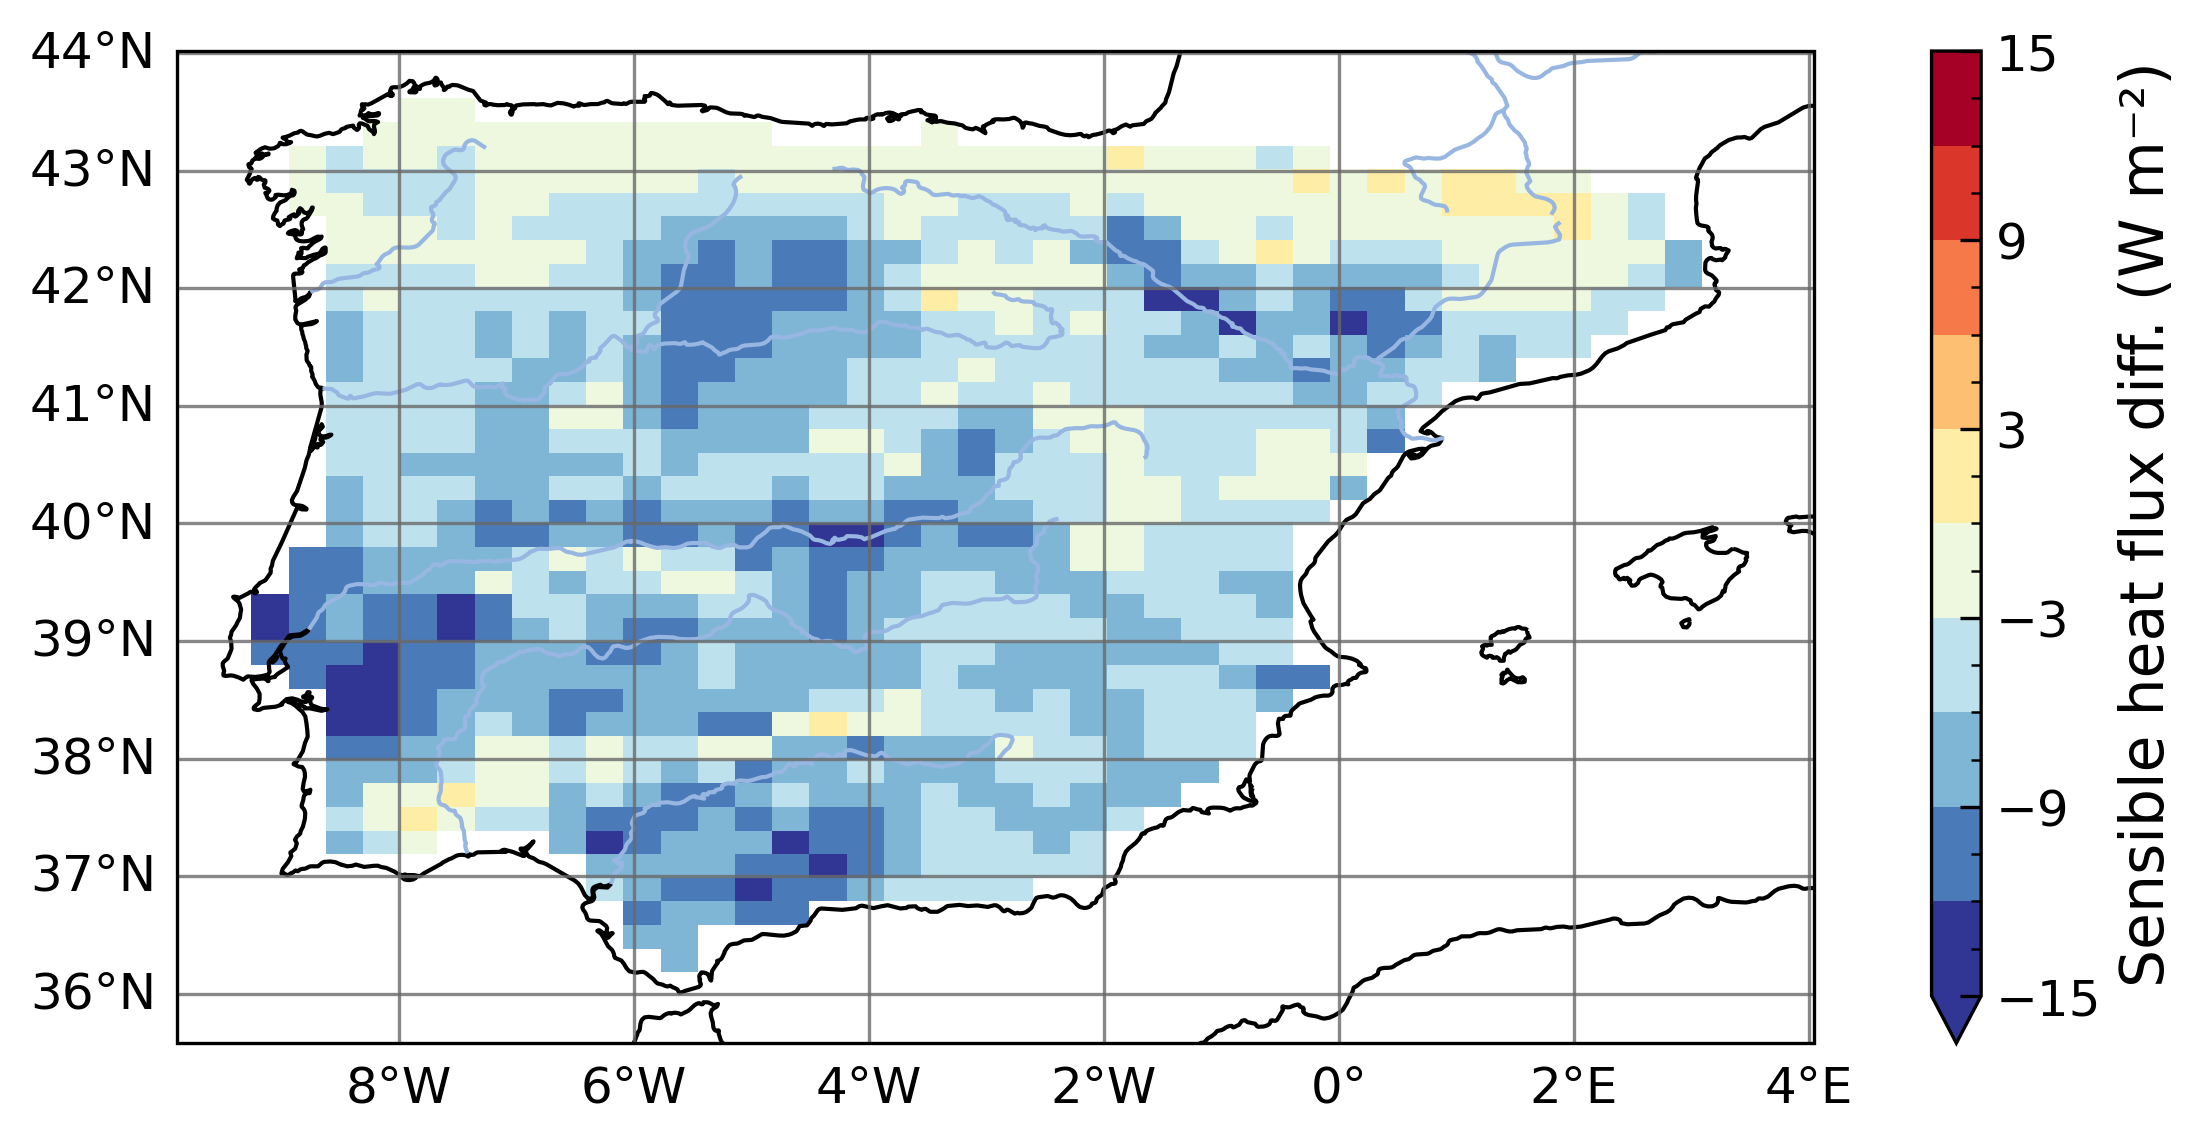
\includegraphics[width=\textwidth]{images/chap4/future/diffmap_fluxsens_futirr.png}
        \end{subfigure} \\

        %q2m
        \begin{subfigure}[b]{0.5\textwidth}
            \caption{}
            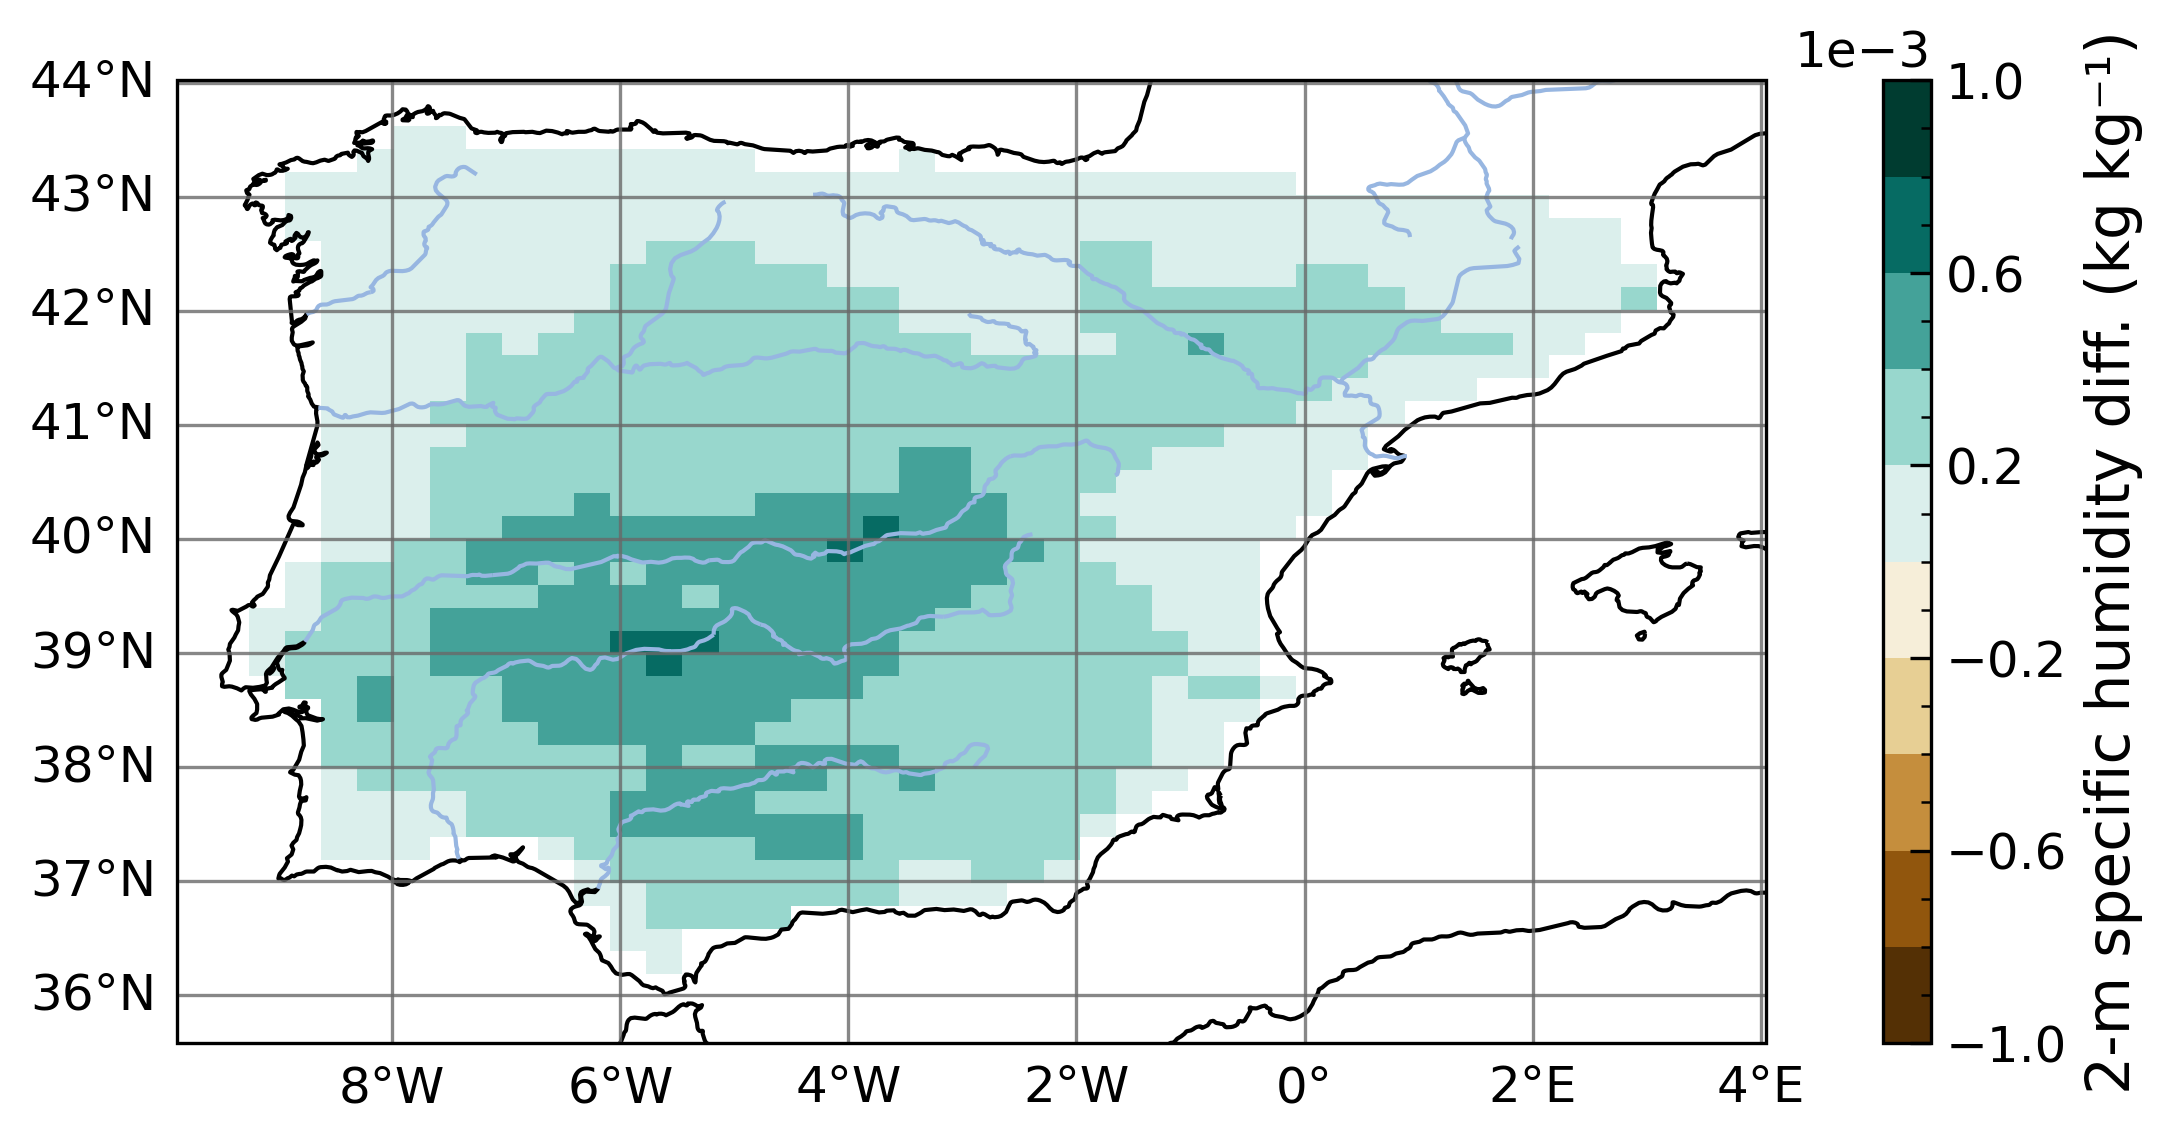
\includegraphics[width=\textwidth]{images/chap4/future/diffmap_q2m_futirr.png}
        \end{subfigure} &
        %rh2m
        \begin{subfigure}[b]{0.5\textwidth}
            \caption{}
            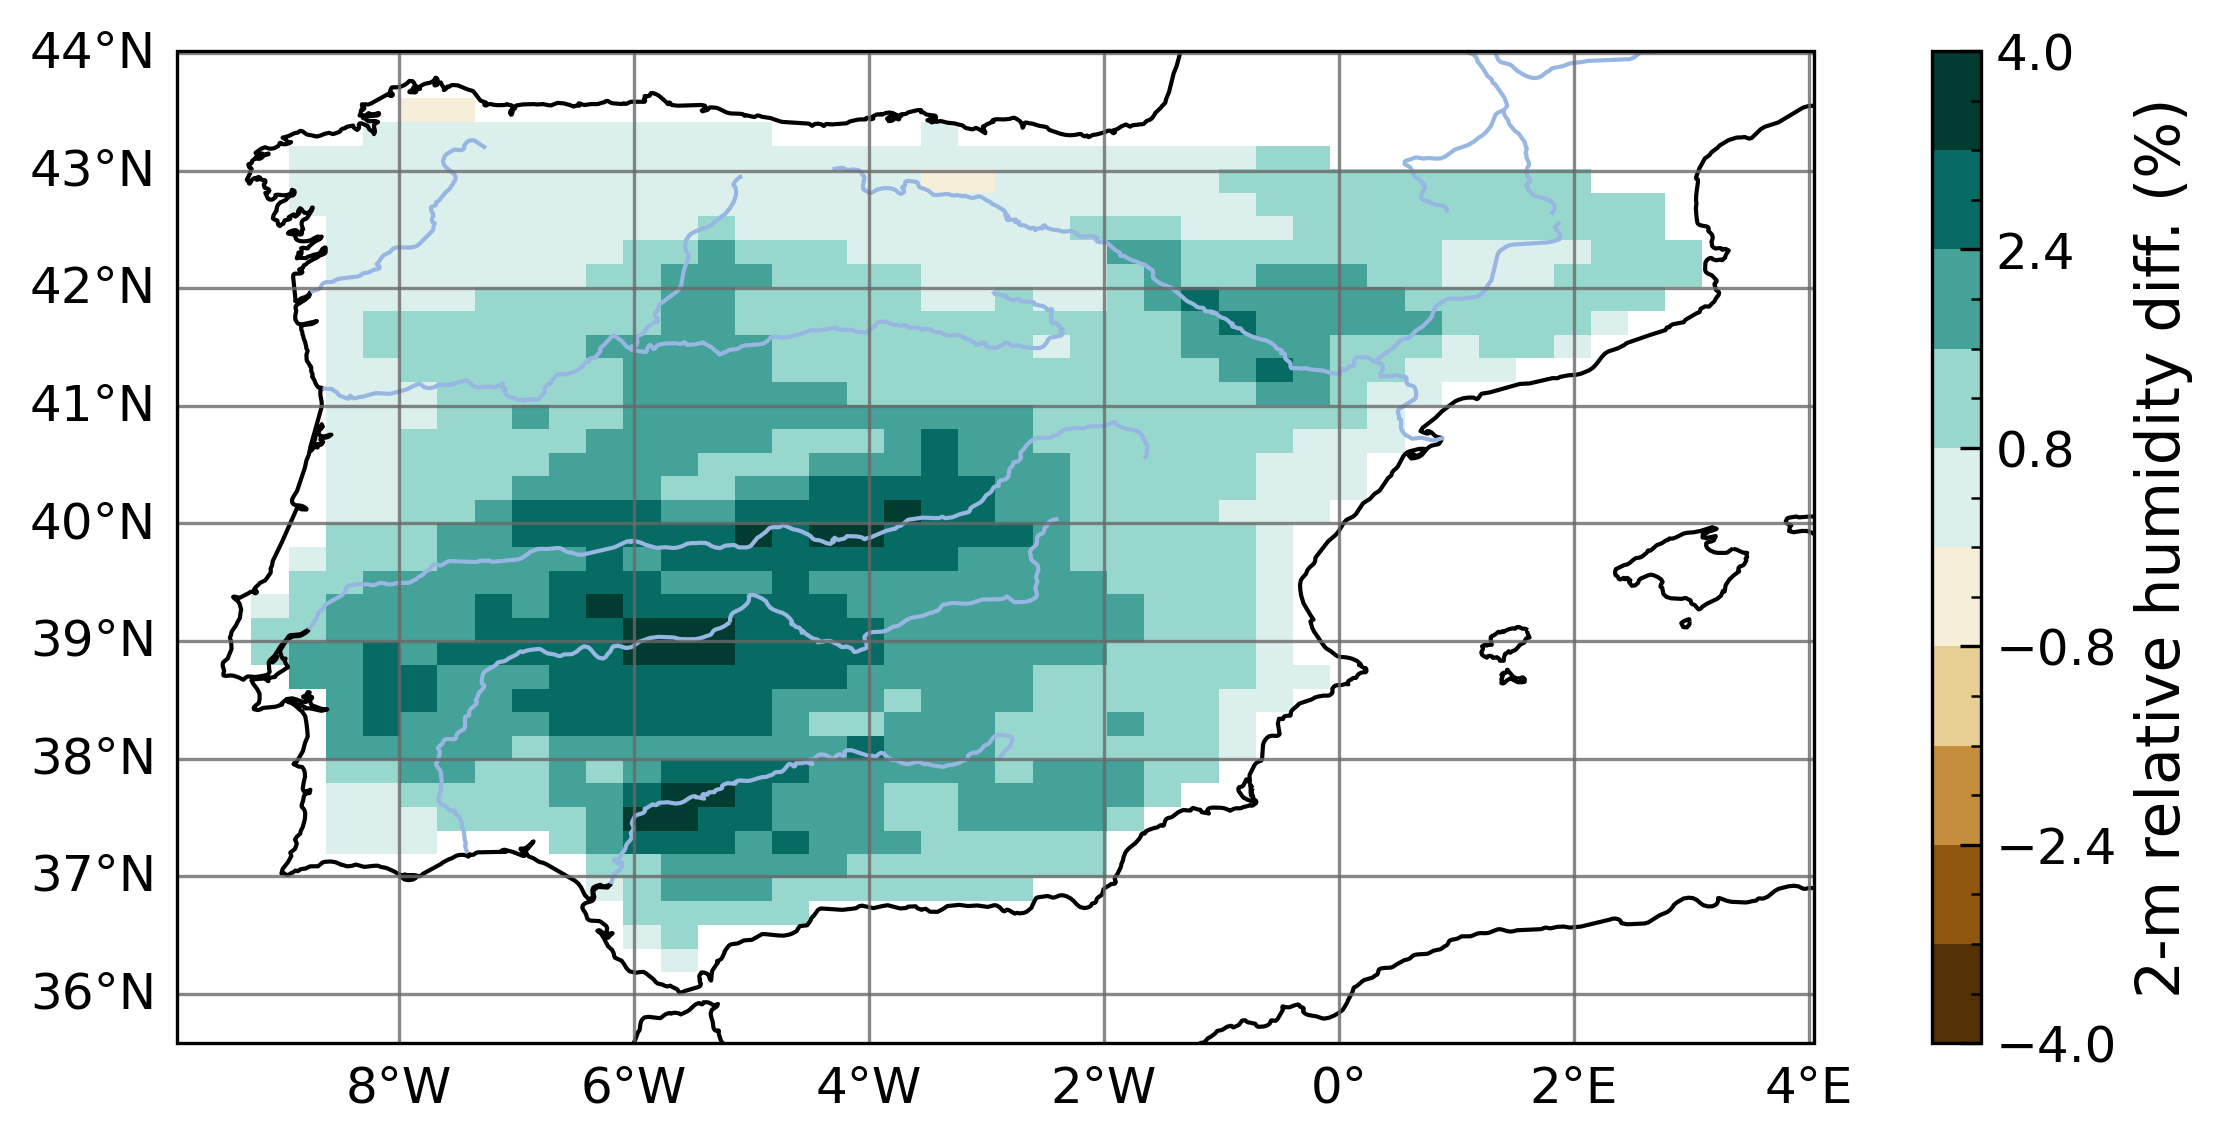
\includegraphics[width=\textwidth]{images/chap4/future/diffmap_rh2m_futirr.png}
        \end{subfigure} \\

        %pblh
        \begin{subfigure}[b]{0.5\textwidth}
            \caption{}
            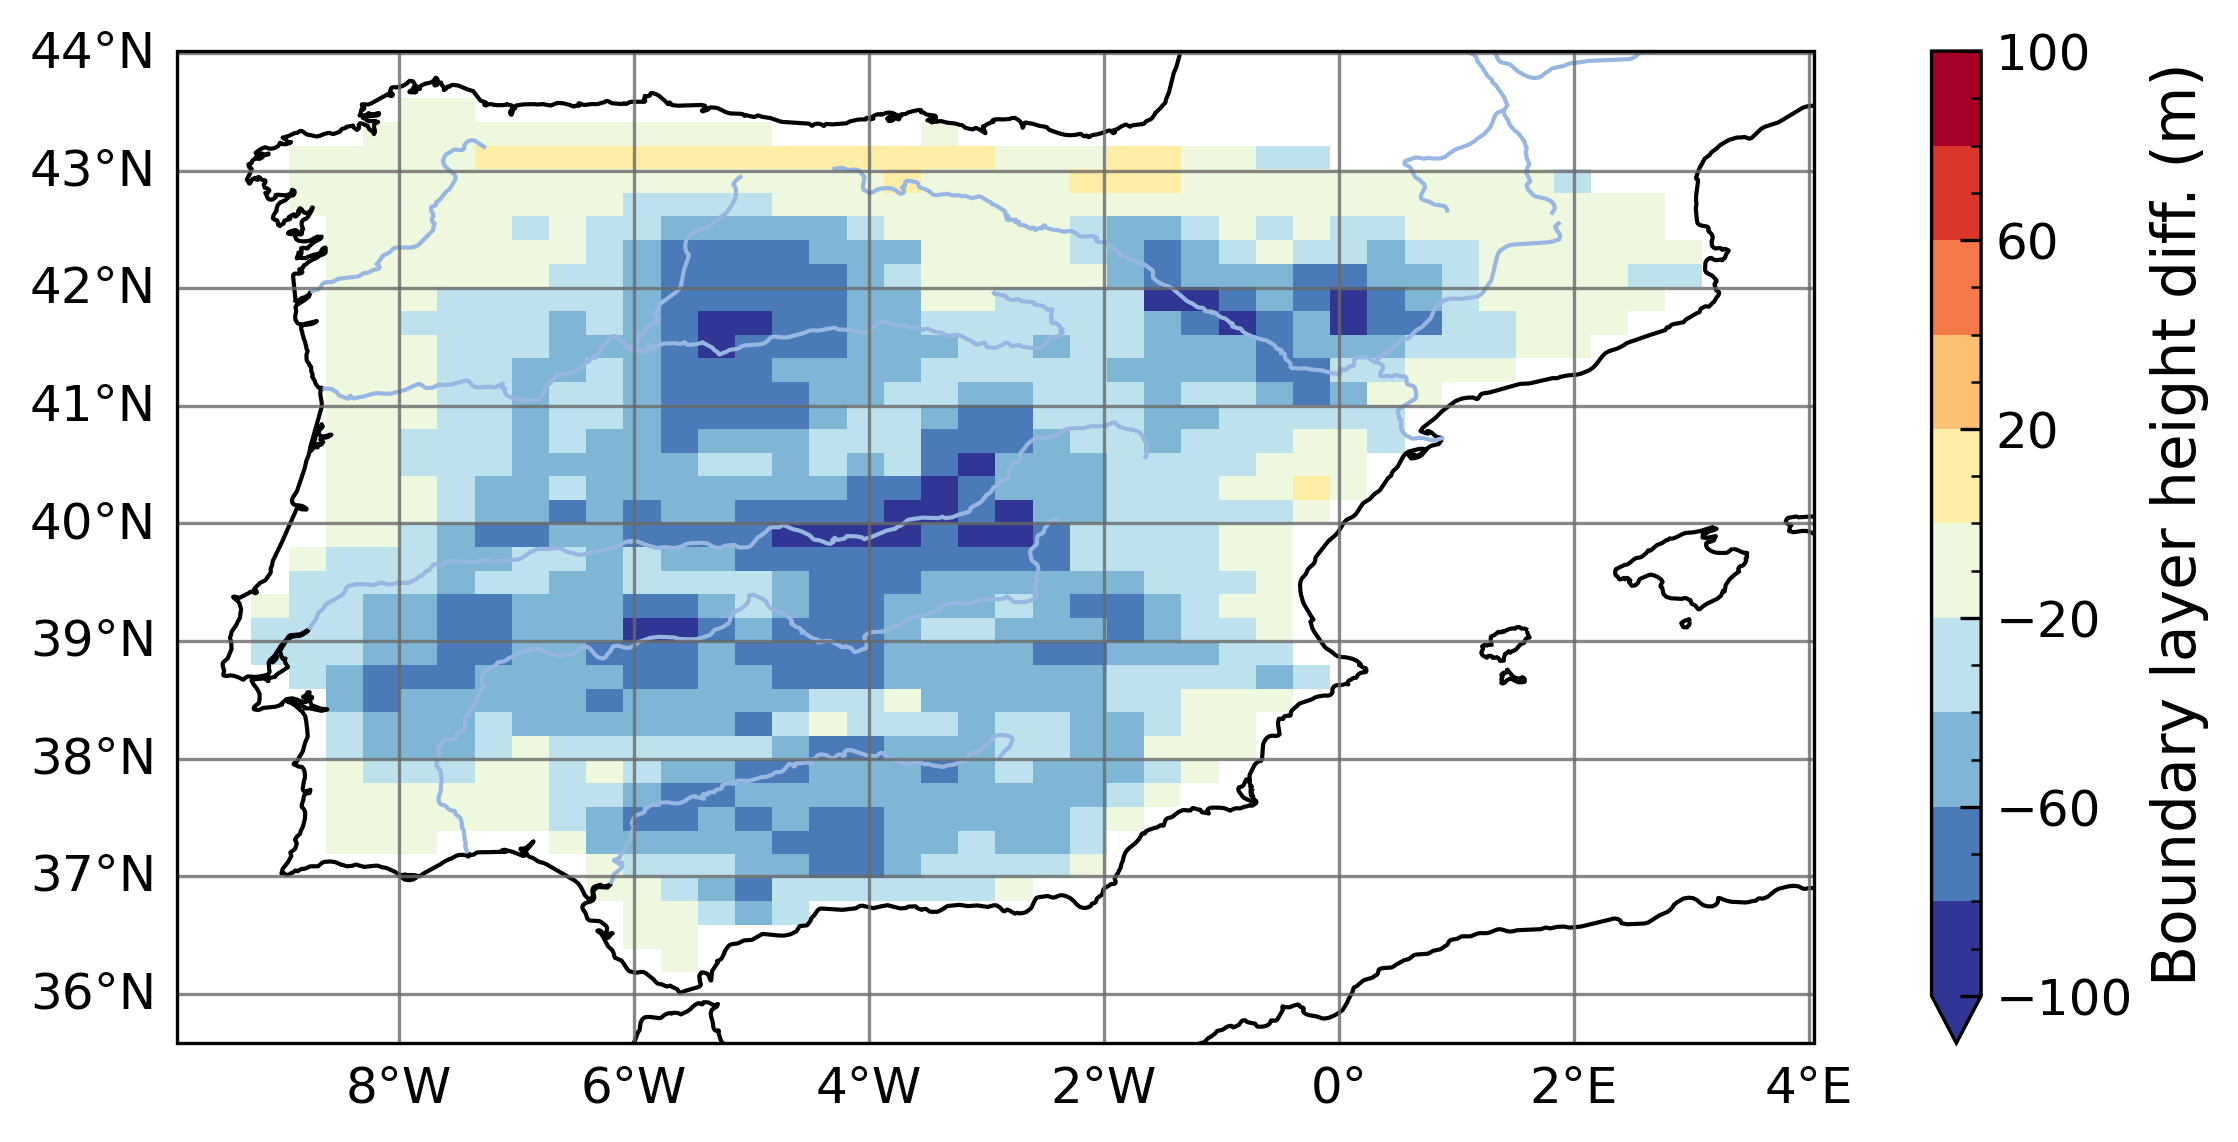
\includegraphics[width=\textwidth]{images/chap4/future/diffmap_s_pblh_futirr.png}
        \end{subfigure} &
        %lcl
        \begin{subfigure}[b]{0.5\textwidth}
            \caption{}
            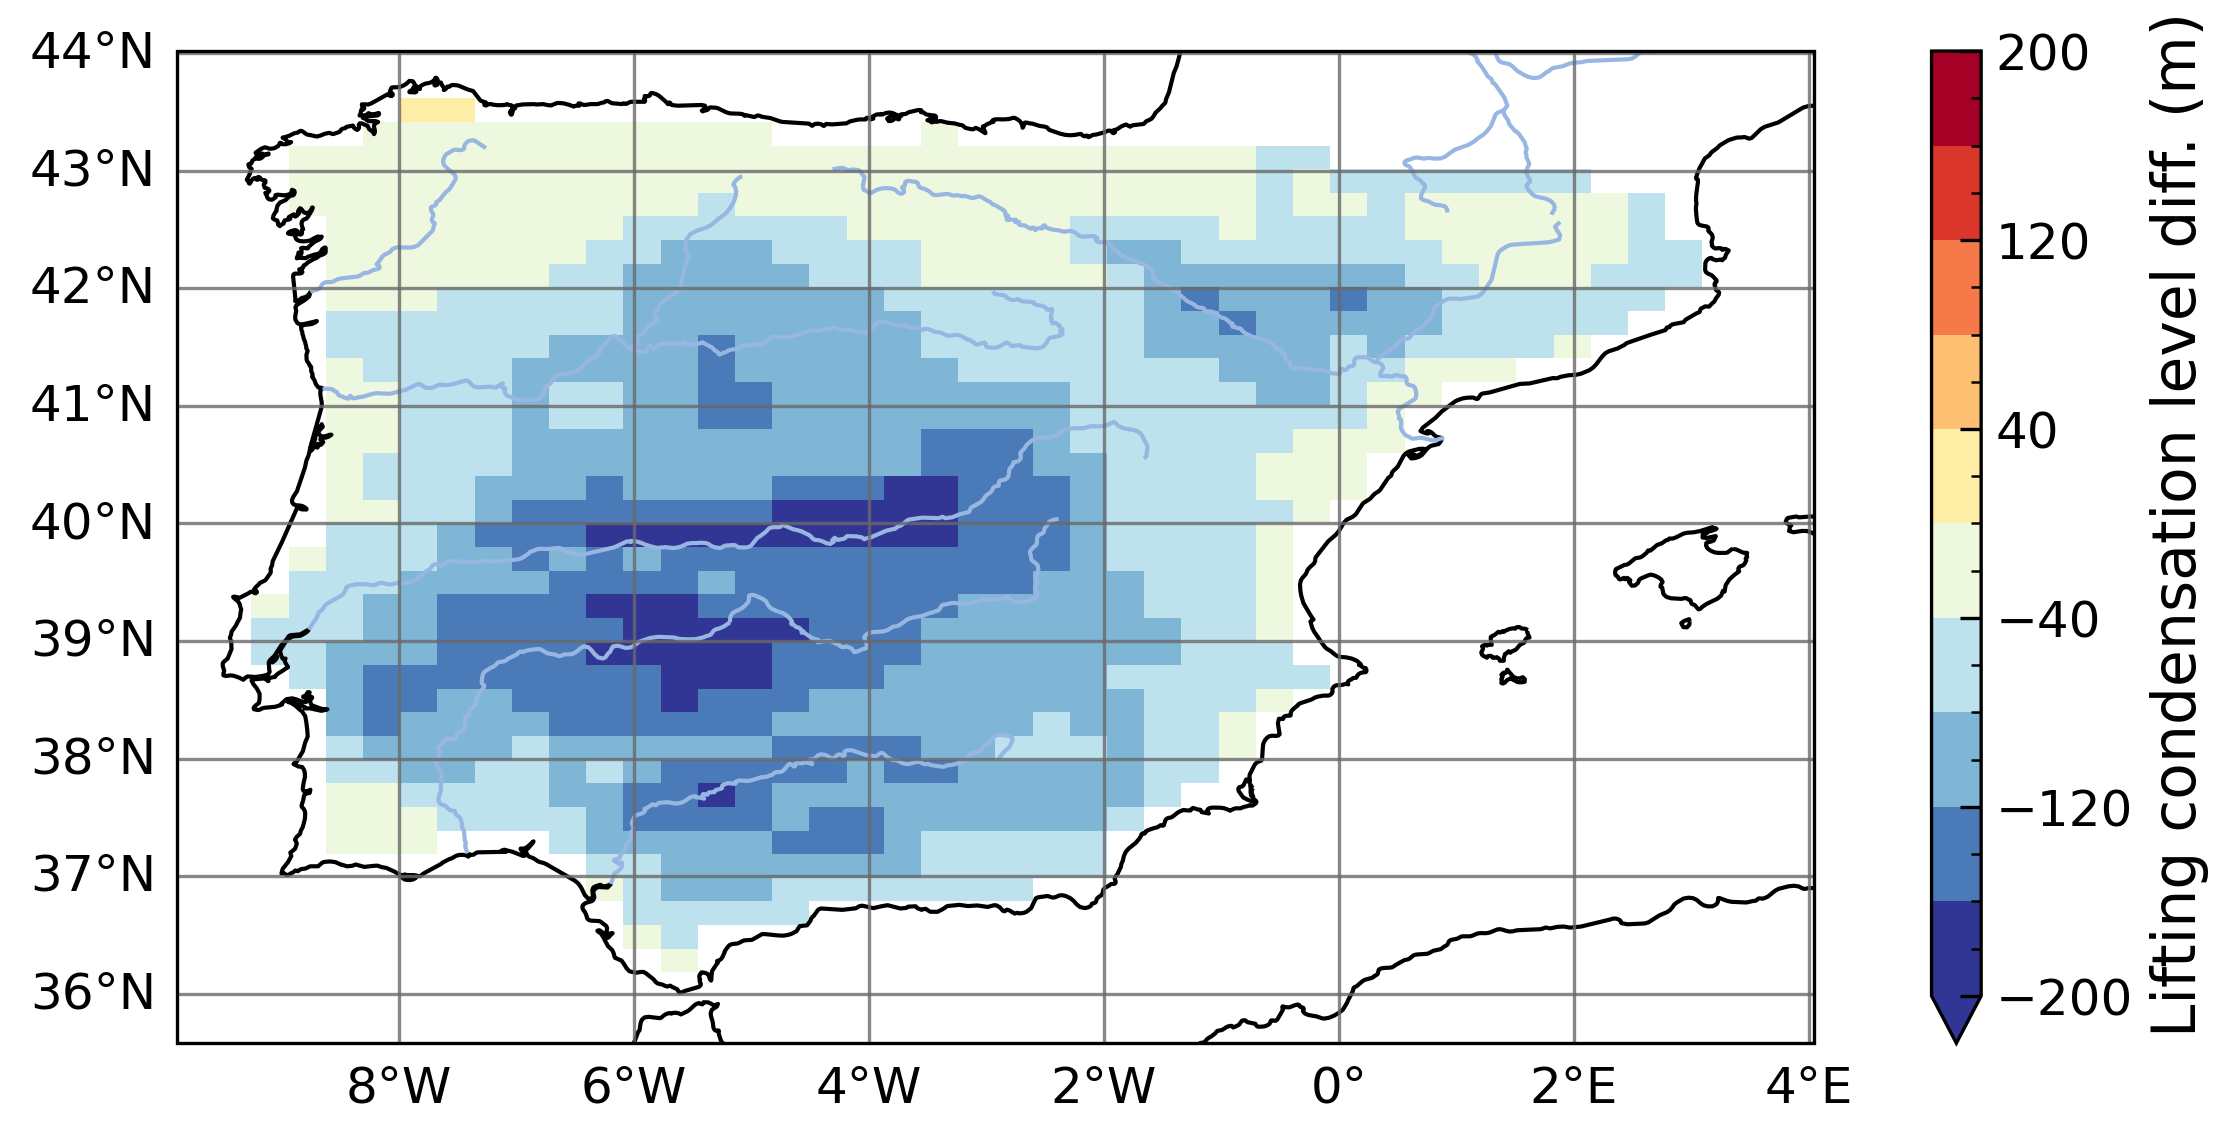
\includegraphics[width=\textwidth]{images/chap4/future/diffmap_s_lcl_futirr.png}
        \end{subfigure} \\
    \end{tabular}
    \caption{}
    \label{fig:diffmaps_future_irr}
\end{figure}

\clearpage

\subsection{Aridification and impact of irrigation}

%figure : maps of aridity index classes for present and future
\begin{figure}[htbp]
    \centering
    %pres, no_irr
    \begin{subfigure}[b]{0.67\textwidth}
        \caption{}
        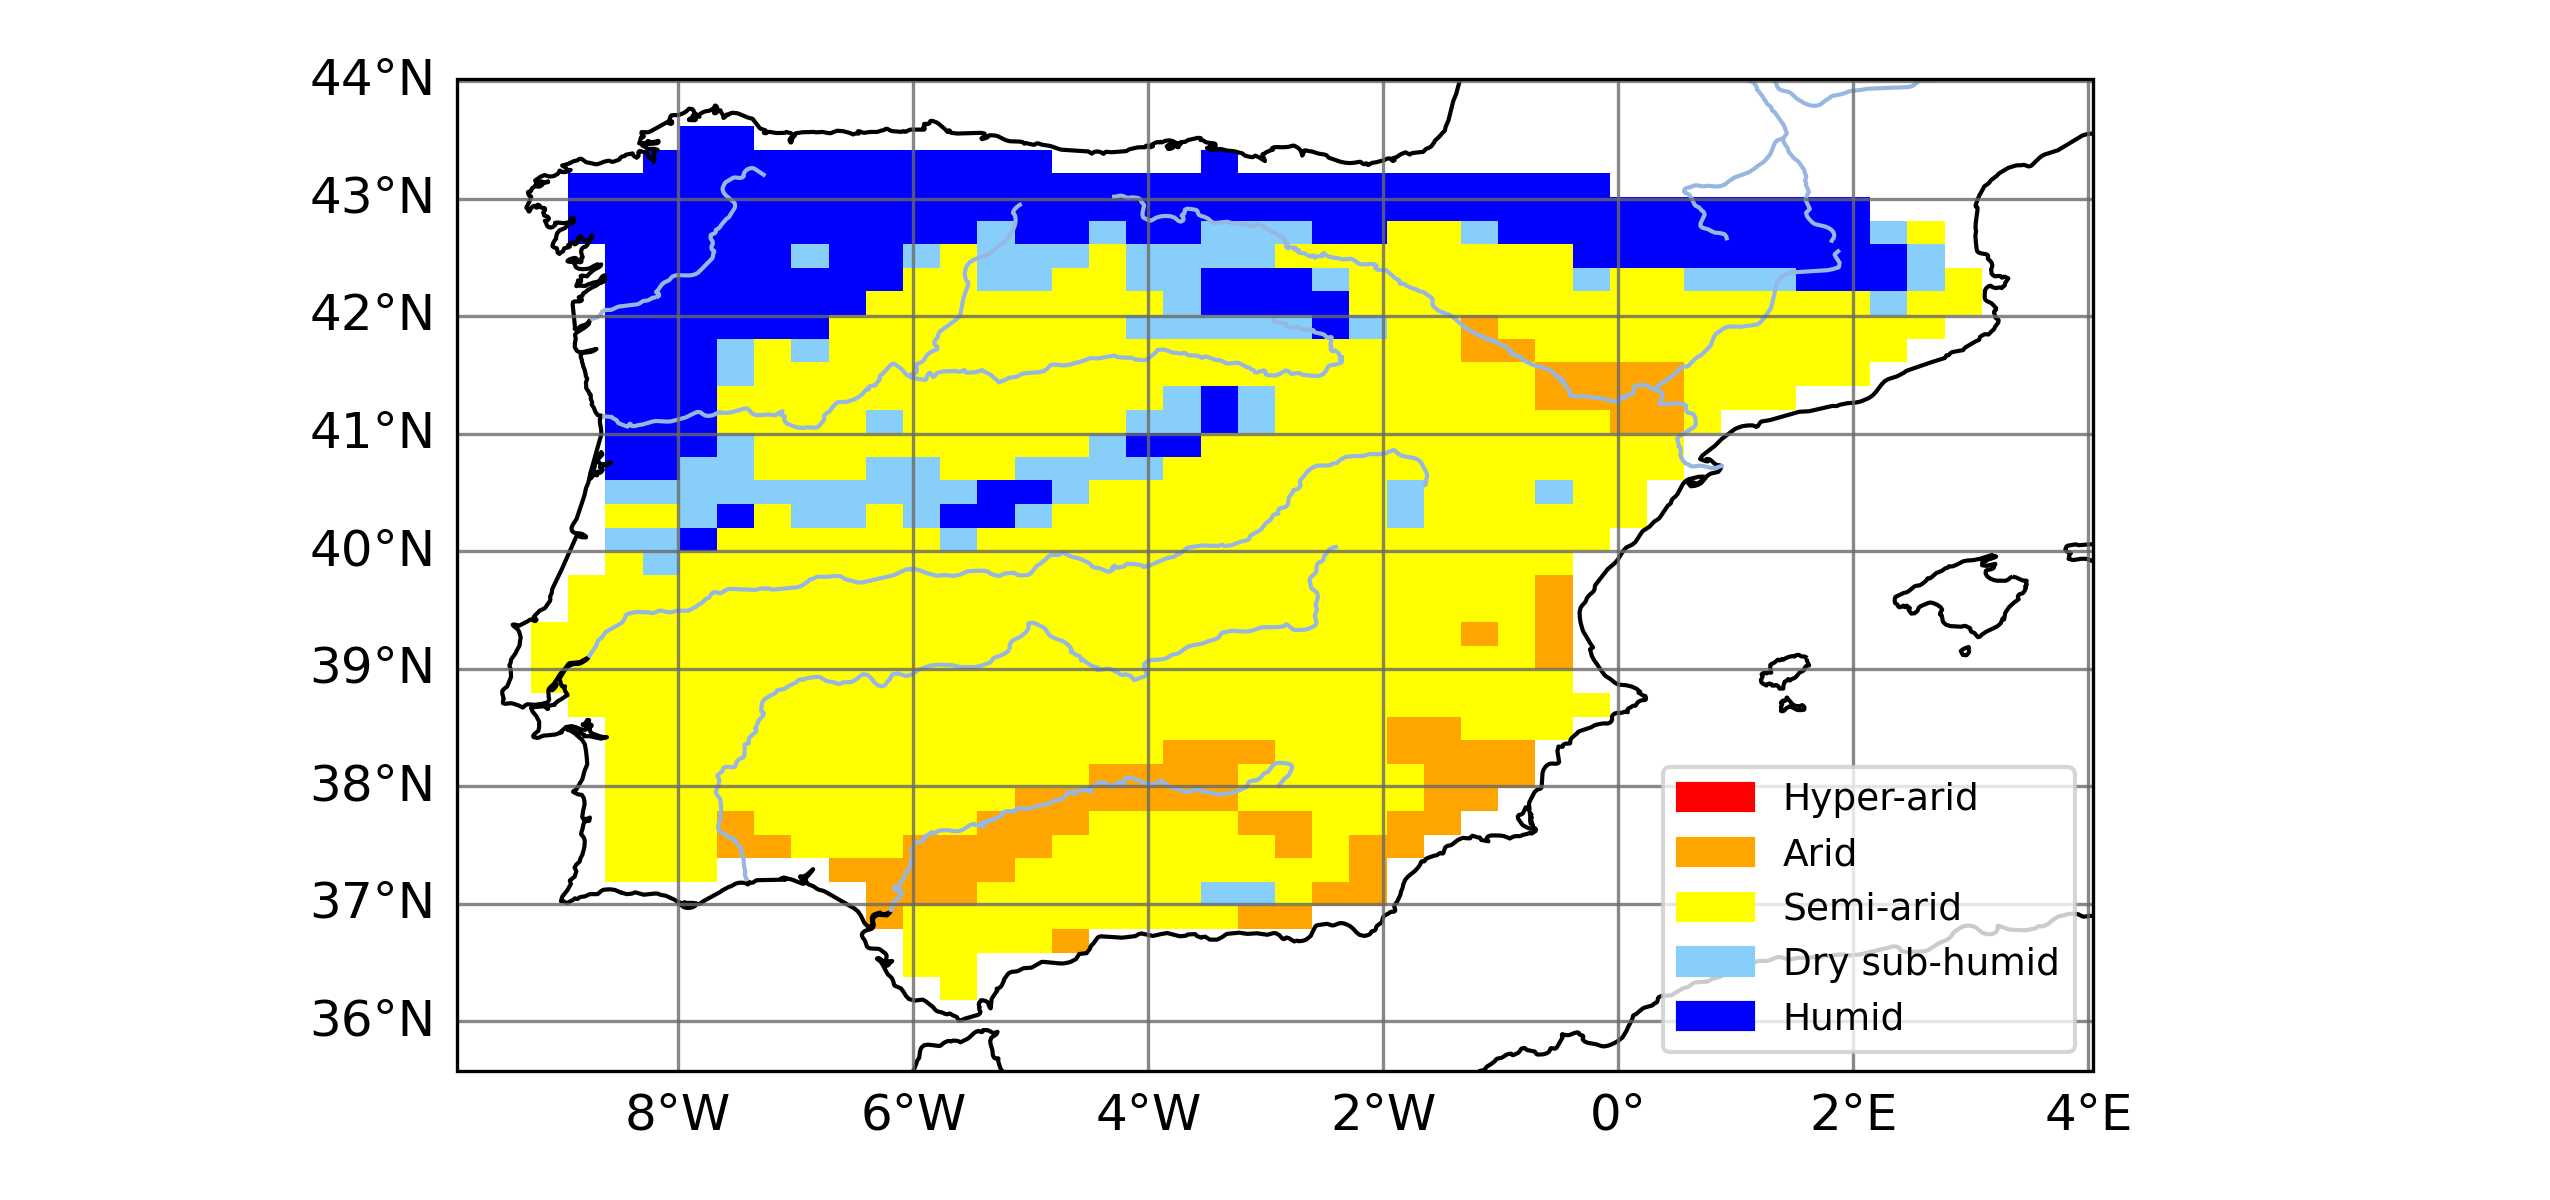
\includegraphics[width=\textwidth]{images/chap4/future/aridity_index_pres_noirr.png}
    \end{subfigure}
    \begin{subfigure}[b]{0.31\textwidth}
        \caption{}
        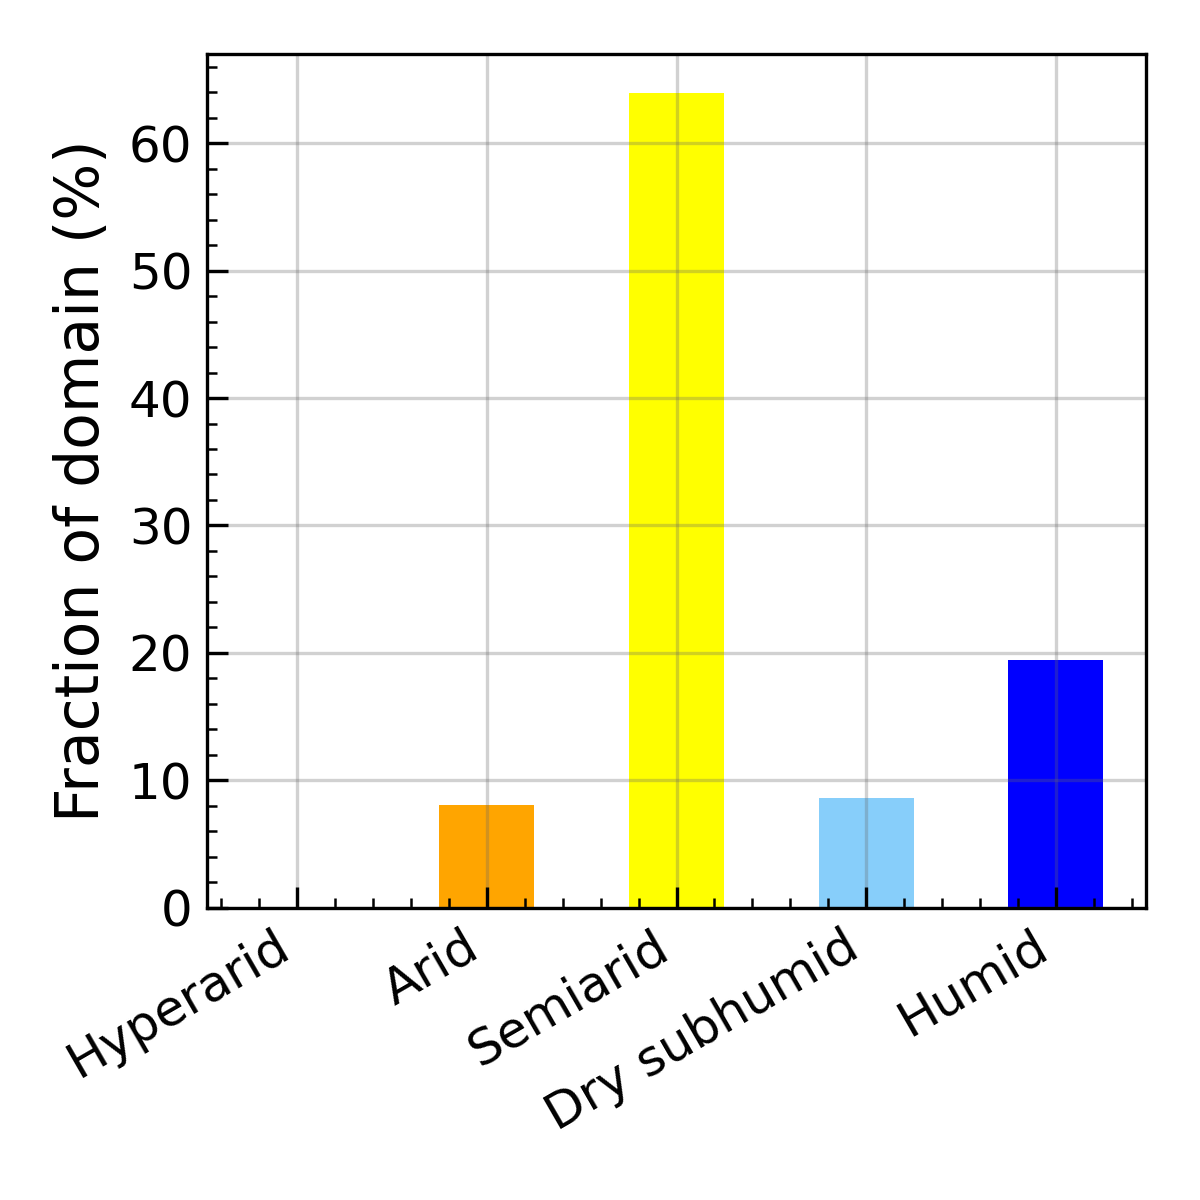
\includegraphics[width=\textwidth]{images/chap4/future/aridity_index_distribution_pres_noirr.png}
    \end{subfigure} \\

    %future, noirr
    \begin{subfigure}[b]{0.67\textwidth}
        \caption{}
        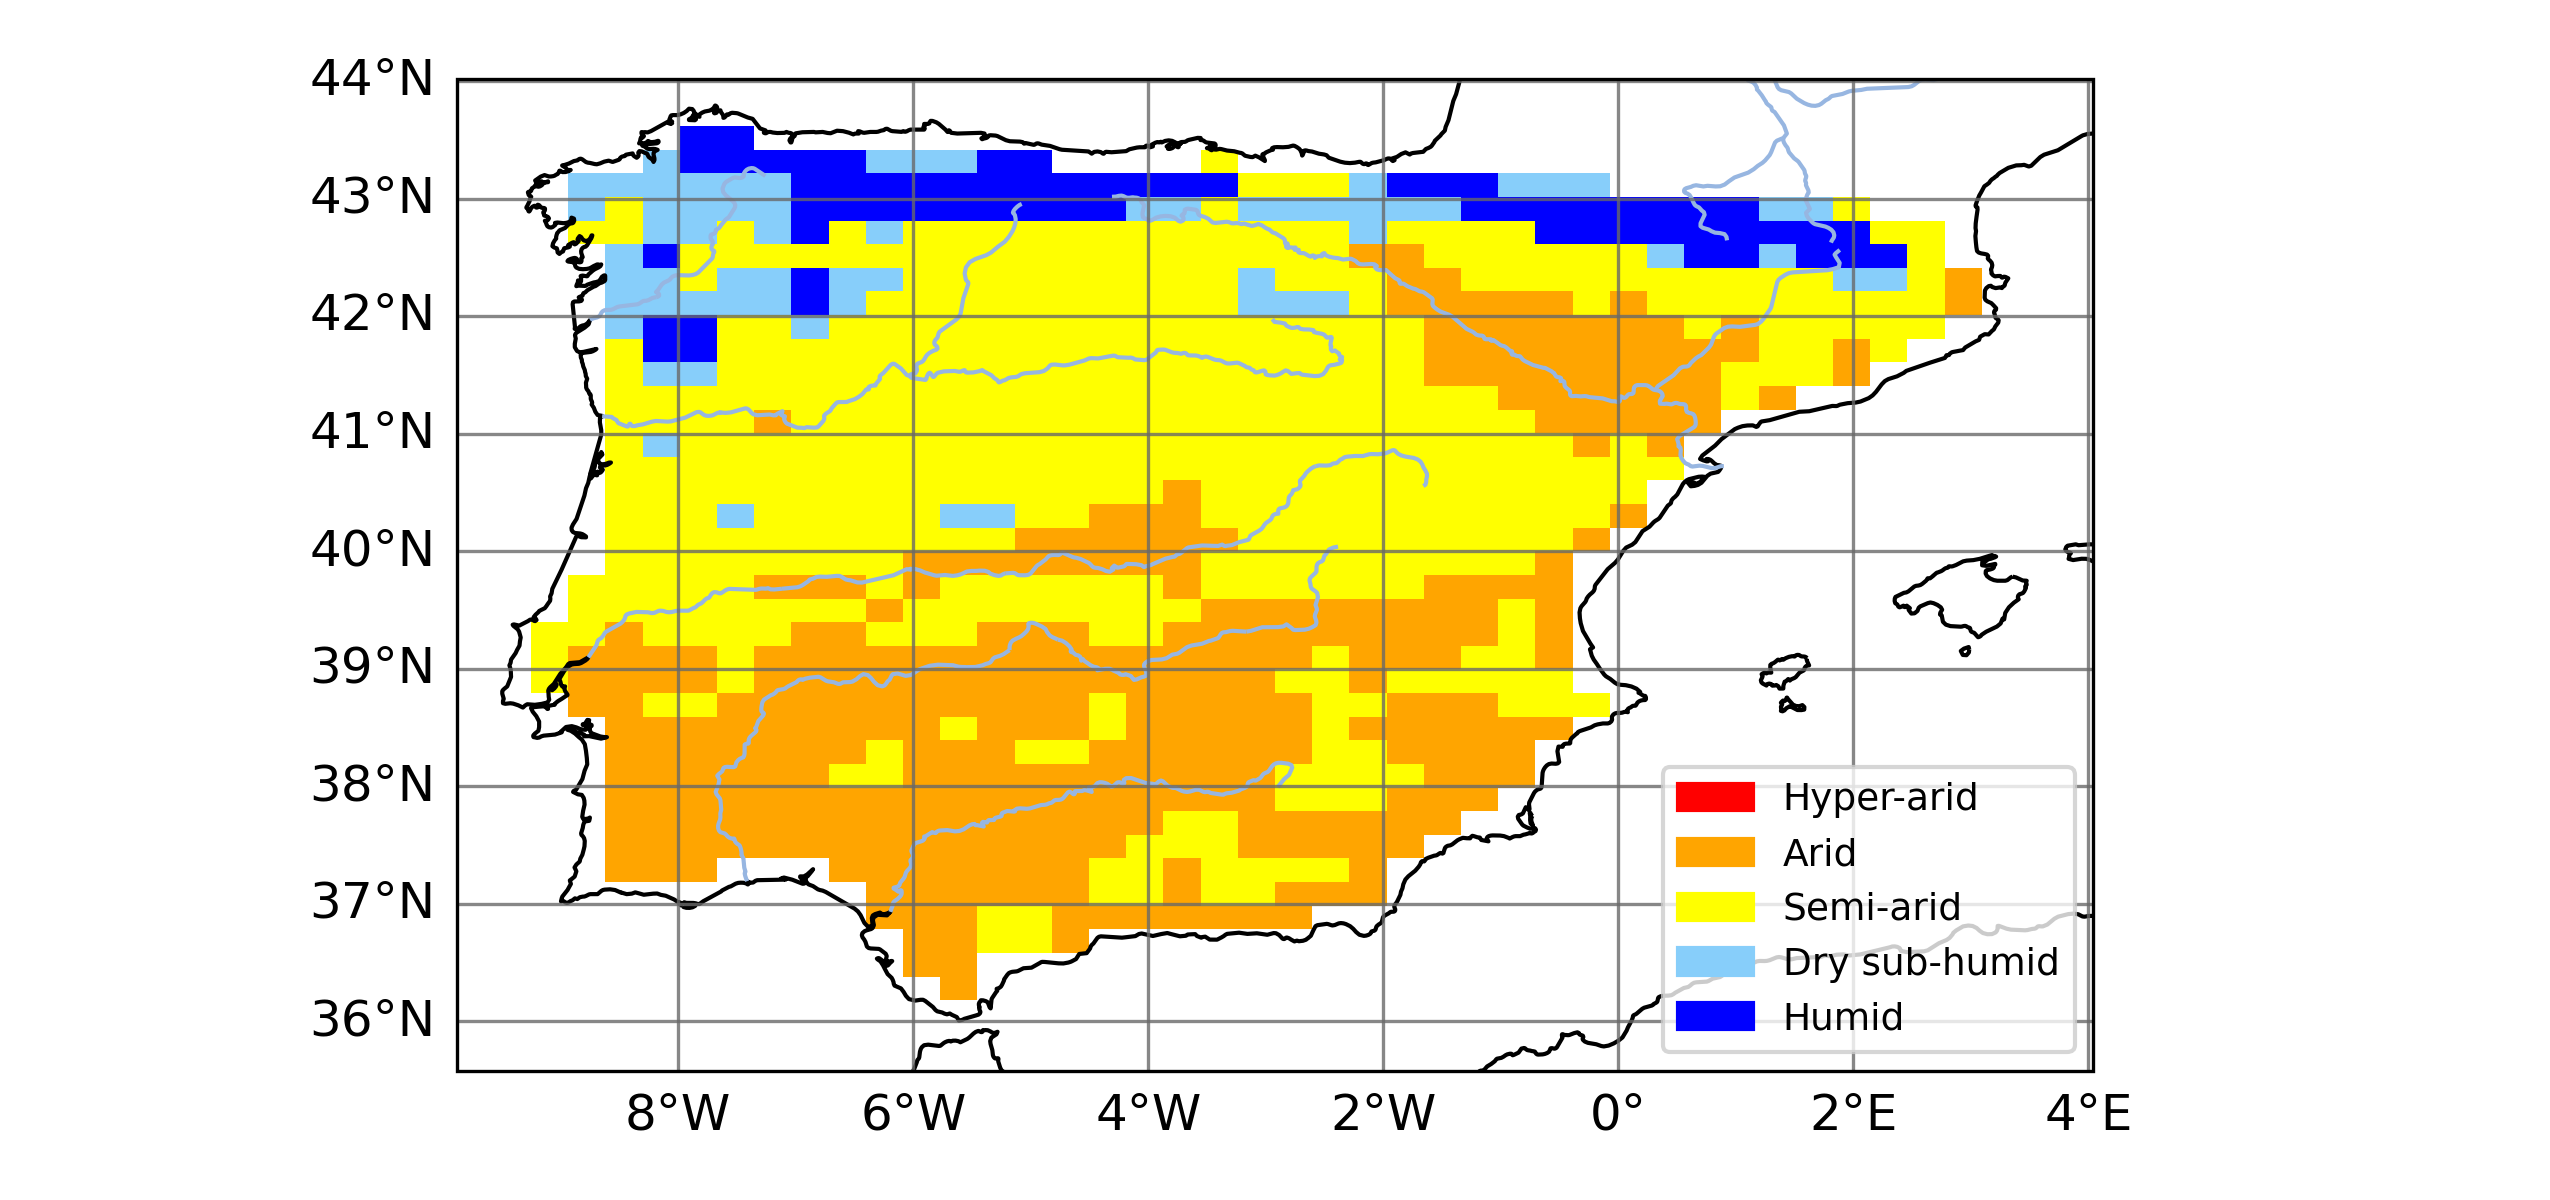
\includegraphics[width=\textwidth]{images/chap4/future/aridity_index_fut_noirr.png}
    \end{subfigure}
    \begin{subfigure}[b]{0.31\textwidth}
        \caption{}
        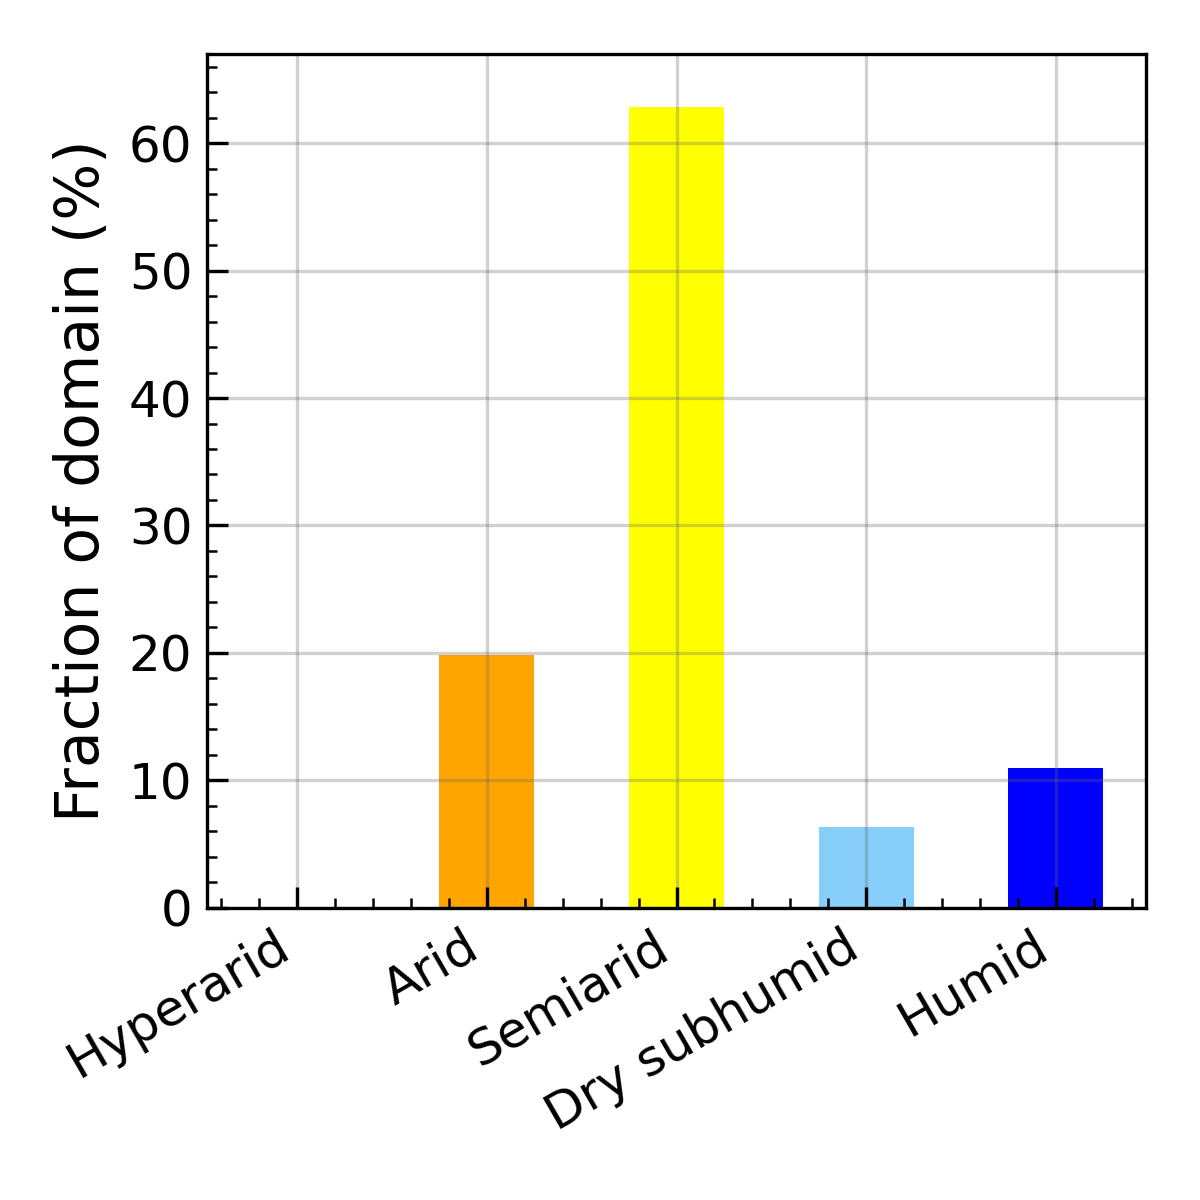
\includegraphics[width=\textwidth]{images/chap4/future/aridity_index_distribution_fut_noirr.png}
    \end{subfigure} \\

    %future, irr
    \begin{subfigure}[b]{0.67\textwidth}
        \caption{}
        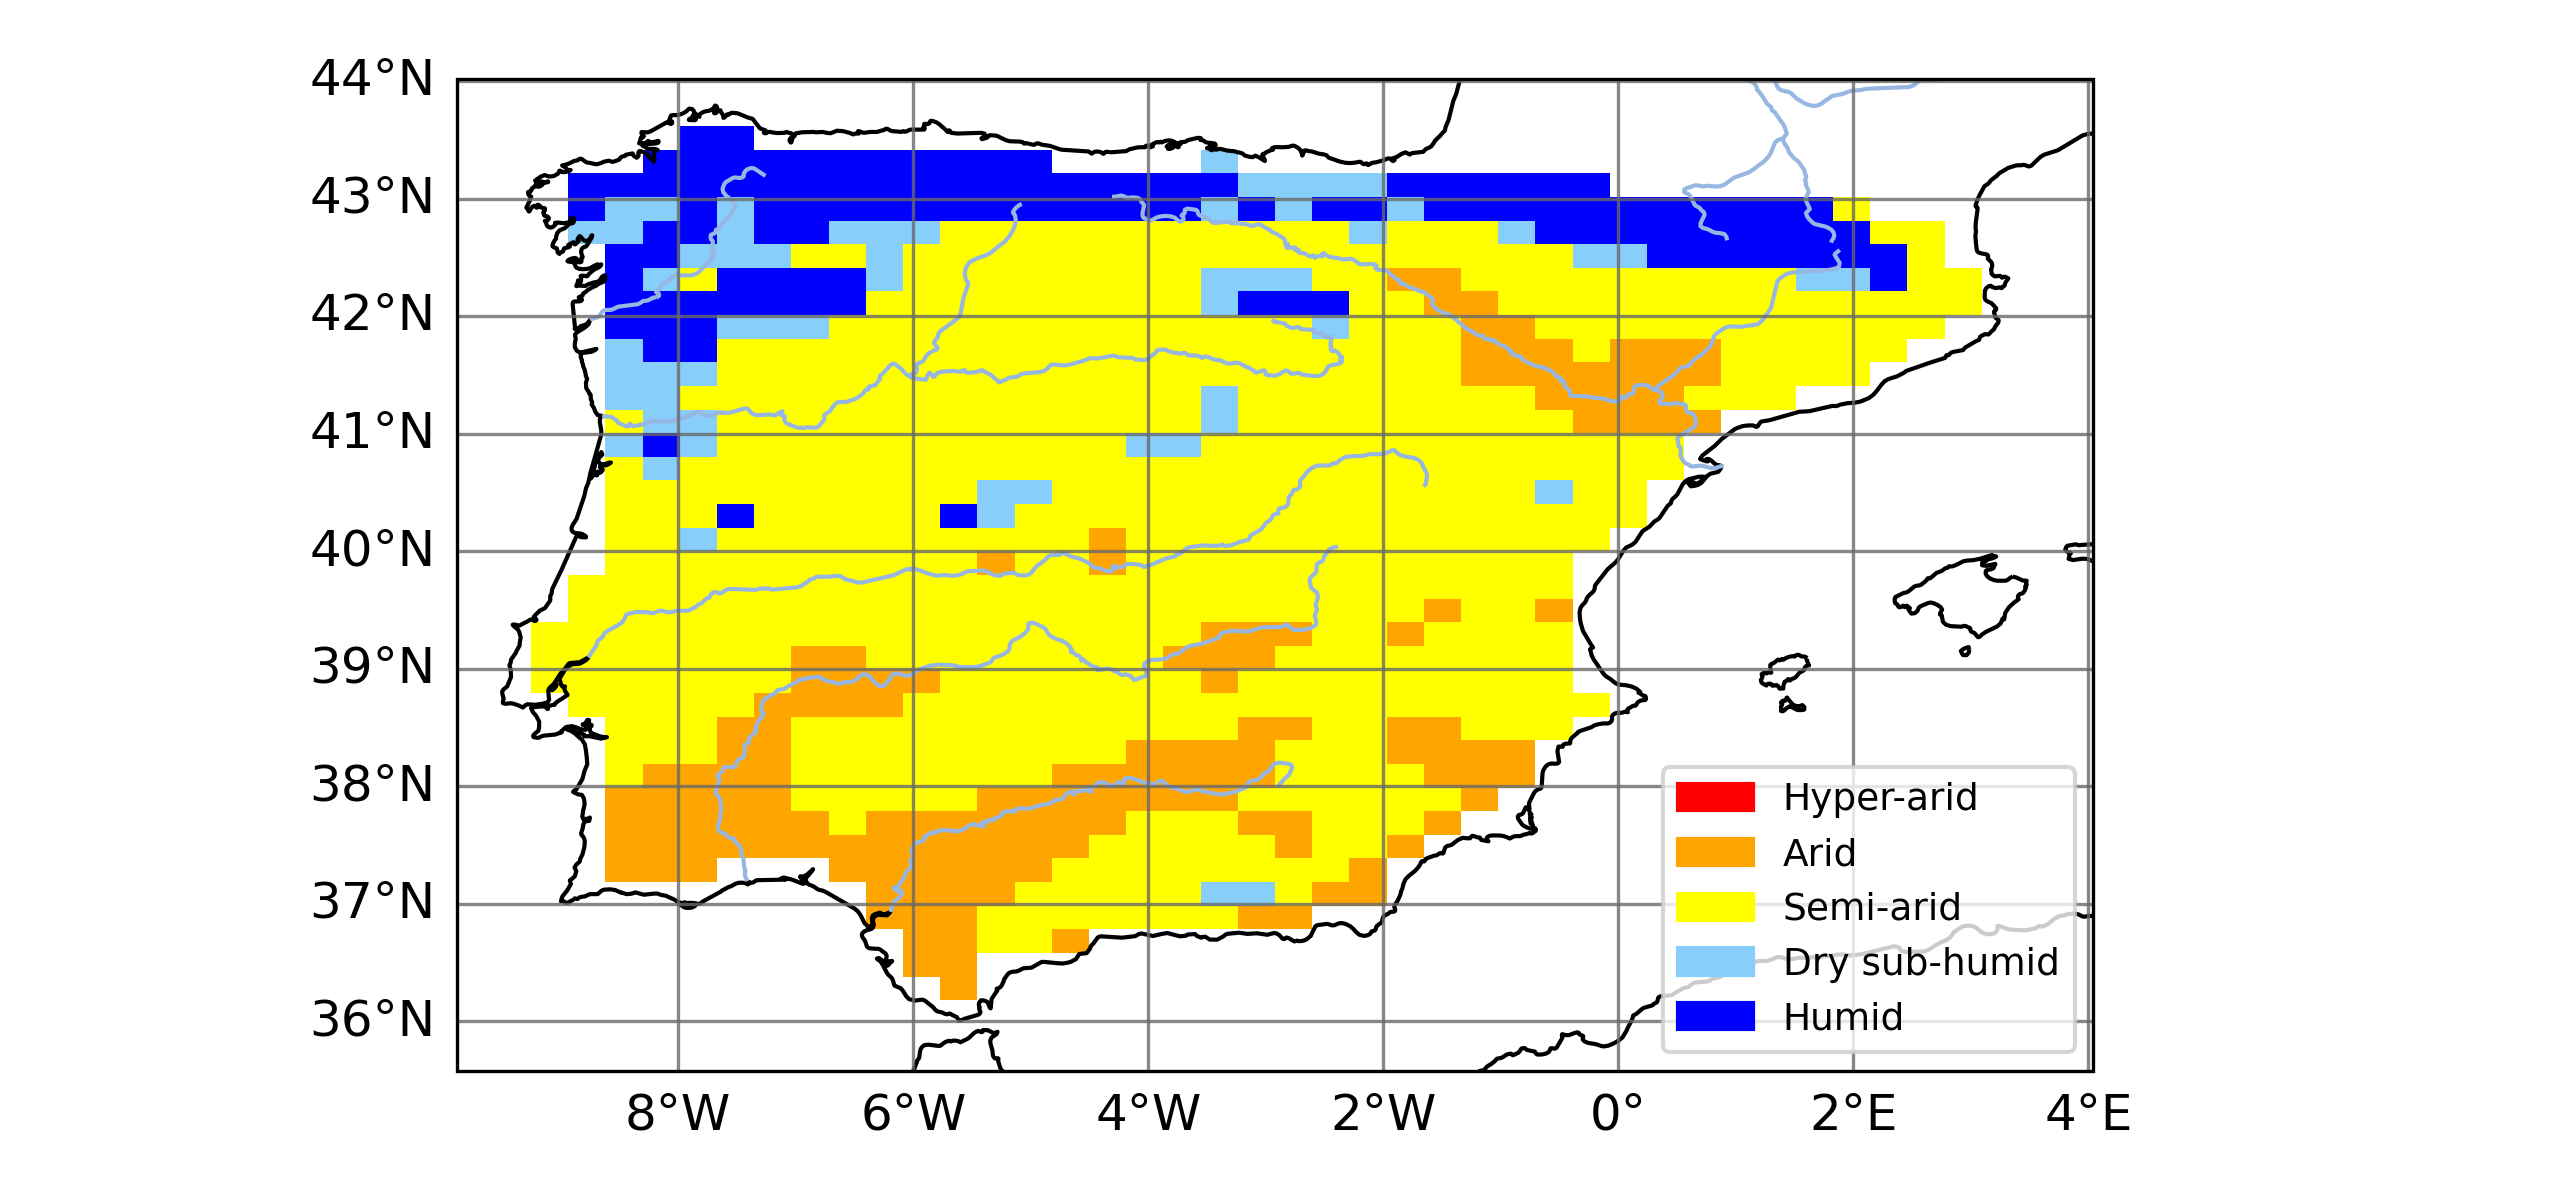
\includegraphics[width=\textwidth]{images/chap4/future/aridity_index_fut_irr.png}
    \end{subfigure}
    \begin{subfigure}[b]{0.31\textwidth}
        \caption{}
        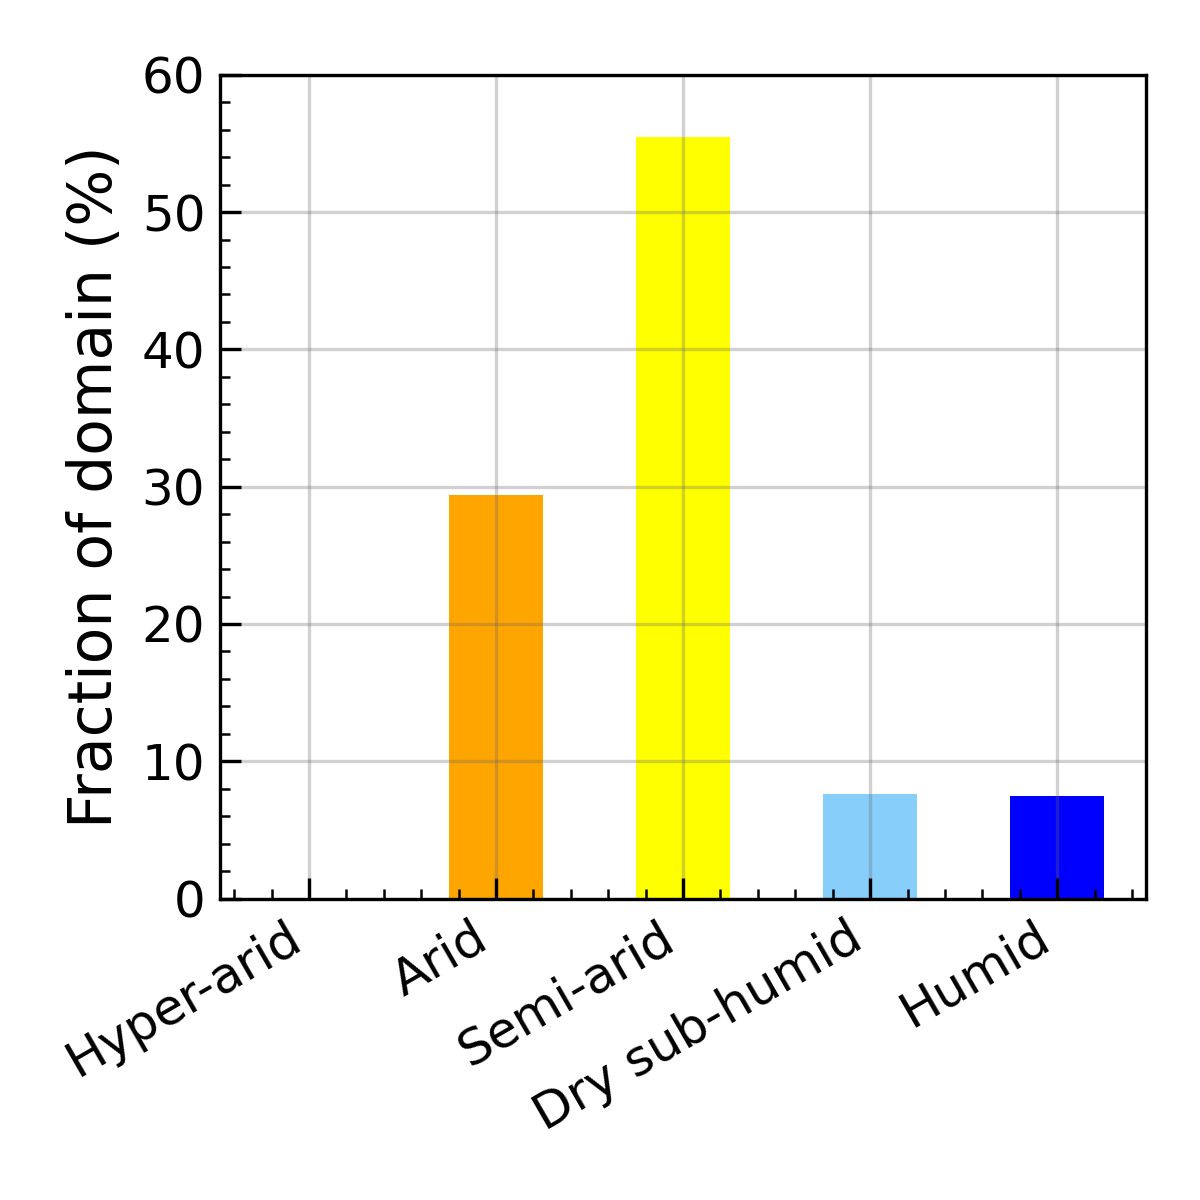
\includegraphics[width=\textwidth]{images/chap4/future/aridity_index_distribution_fut_irr.png}
    \end{subfigure}
    \caption{}
    \label{fig:aridity_index_v2}
\end{figure}
